 %美赛模板:正文部分

\documentclass[12pt]{article}  % 官方要求字号不小于 12 号,此处选择 12 号字体
% \linespread{1.1}
% \bibliographystyle{plain}
% 本模板不需要填写年份,以当前电脑时间自动生成
% 请在以下的方括号中填写队伍控制号

\usepackage[2412704]{easymcm}  % 载入 EasyMCM 模板文件

\problem{C}  % 请在此处填写题号

\usepackage[english]{babel}

% \usepackage{mathptmx}  % 这是 Times 字体,中规中矩 
\usepackage{palatino}  % mathpazo 这palatino是 COMAP 官方杂志采用的更好看的 Palatino 字体,可替代以上的 mathptmx 宏包
\usepackage{pdfpages}
\usepackage{longtable}
\usepackage{graphicx}
\usepackage{caption}
\usepackage{fancyhdr}
\usepackage{booktabs}
\usepackage{hyperref}
\usepackage{tabu}
\usepackage{algorithm}
\usepackage{pdfpages}
\usepackage{lastpage}  % To reference the last page before the PDF is included
\usepackage{algorithmic}
\usepackage{threeparttable}
\usepackage{listings}
\usepackage{multicol}
\usepackage{paralist}

\graphicspath{{img/}}          % 此处{img/}为相对路径,注意加上“/”
 \let\itemize\compactitem
 \let\enditemize\endcompactitem

\newcommand{\upcite}[1]{\textsuperscript{\textsuperscript{\cite{#1}}}}
\title{Momentum Quantifier (MoQ): Proving the "Big Mo" is Real in Tennis}  % 标题

% 如需要修改题头(默认为 MCM/ICM),请使用以下命令(此处修改为 MCM)
%\renewcommand{\contest}{MCM}

 %文档开始
\begin{document}

% 此处填写摘要内容
\begin{abstract}
    
Yes, the Big Mo ("Big Momentum") is real.

% 美赛论文中无需注明关键字。若您一定要使用,
% 请将以下两行的注释号 '%' 去除,以使其生效
\vspace{5pt}  %mm	毫米	1 mm = 2.845 pt   pt 点	1 pt = 0.351 mm;此处为Keywords与Abstract正文额外相隔的距离(1.5cm)
\textbf{Keywords}: Feature Engineering, Logistic Regression, Dynamic Model

\end{abstract}

\maketitle  % 生成 Summary Sheet


% 生成目录

\tableofcontents  



% Chapter 1: Introduction

\section{Problem Background}
If you are a fan in competitive sports games like tennis, you might have heard a lot of the word “Momentum”. When a player has momentum, they seem to control the dominance of the match, wielding the match's rhythm and flow. Novak Djokovic, a record-breaking tennis player, described this in his saying: “… if you have the mental ability to stay strong, stay patient and confident and just have belief in the right moments, then you get a win, you know.”

However, momentum is not stationary; you probably have witnessed momentum being lost or stolen from a player during a match, entirely changing the outcome. Momentum can switch to the other player within the blink of an eye and stun unsuspecting players and spectators. This is especially spectacular during the 2023 Wimbledon Gentlemen’s final between Carlos Alcaraz and Novak Djokovic (Figure 1). In this match, Djokovic completely dominated the first set with a score of 6 – 1, displaying enormous momentum. However, this quickly shifted to Alcaraz in the third set, where he won 6 - 1, before Djokovic regained control in the fourth set with a 6 - 3 win. Finally, in the late stages of the fifth set, the momentum swung once again, and Alcaraz secured victory with a score of 6 - 4.

But where \textbf{exactly} did that momentum come from? Despite its recognized impact, momentum has remained largely a qualitative factor and rooted in the subjective experience of spectators and self-perception of athletes. The question, then, is whether this intangible force can be analyzed and systematically understood through mathematical methods. If this proves feasible, it has the potential to greatly enhance the strategies used by competitive tennis players and coaches and, by extension, athletes and coaches in various sports.

\begin{figure}[htbp]
	\centering
	\begin{minipage}{0.5\textwidth}
	\centering  %图表居中

\includegraphics[width=.95\textwidth]{carlos-alcaraz.jpg} %图片的名称或者路径之中有空格会出问题 
\caption{Carlos Alcaraz (Left) and Novak Djokovic (Right) at Wimbledon \cite{1}} % 图片标题 
\label{fig:Fire Situation} % 图片标签,可以不写
	\end{minipage}\hfill
	\begin{minipage}{0.45\textwidth}
	\centering  %图表居中
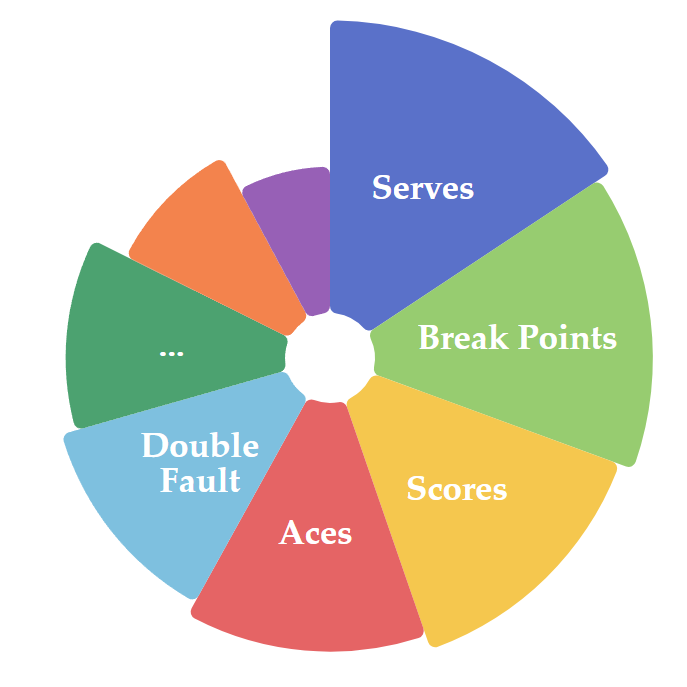
\includegraphics[width=.6\textwidth]{data-given.png} %图片的名称或者路径之中有空格会出问题 
\caption{Data Aspects Provided by \textit{Wimbledon\_featured\_matches.csv}} % 图片标题 
\label{fig:Fire Situation} % 图片标签,可以不写
	\end{minipage}
\end{figure}

\section{Problem Analysis: What is Momentum?}

Momentum is often seen as a phenomenon that a player is playing exceedingly well at a time in the match. And because it its a \textit{phenomenon}, it should be an outcome of a wide range of factors, including psychological states, like confidence and mental toughness, to external conditions like the current state of the match. To analyze and build a robust model that measures the momentum of players in competitive tennis, it is crucial to uncover and model these factors extensively. Specifically, our model should be capable of completing the following tasks:

\begin{enumerate}[\bfseries (1)]
	\setlength{\parsep}{0ex} %段落间距
	\setlength{\topsep}{2ex} %列表到上下文的垂直距离
	\setlength{\itemsep}{1ex} %条目间距
	\item Evaluate the quantitative degree how one player is performing better than the other player at any given point in the match, and illustrate the changes of such performance difference in visual representation.
	\item Based on extensive factors, including the flow of match, the model should quantify the concept of "momentum" in tennis matches, and identify potential indicators that could predict shifts in momentum. To address the coach’s skepticism, the model needs to be compared to a null model that assumes outcomes are random (e.g., based on point-by-point win probabilities without momentum).
	\item Finally, the developed "momentum" model should be tested on other matches from the different matches, including women's matches, to exhibit its predictive accuracy and generalizability, and identify any limitations or additional factors that may need to be incorporated. 
\end{enumerate}

\subsection{Capturing the Flow of Match}
To compare the performance ratings between the two players, we can use the data provided in \textit{Wimbledon\_featured\_matches.csv} that describe the explicit match information, such as whether a player was serving or at a break point, etc. (shown in Figure 2); but we also need to consider other implicit information that has significant impact on the state of the match, for example, whether a player has a high scoring streak. Other unimportant information, potentially the speed of the serve, needs to be neglected to ensure model's simplicity and robustness. This inherently requires \textbf{feature engineering}: to extract and construct feature variables that capture both explicit and implicit aspects that control the flow of the match.

Since our model aims to dynamically assess the match's state as it evolves, it requires a granular focus on the state of the game, taking into account both minor and major developments. For example, the player may have a lead in games won, but when the other player just scored a break point, that player could be performing much better at that specific time. Therefore, to scope the data to recently played points, the \textbf{sliding window} technique can be employed; to handle older scores and progressively update the model as the match goes on, introduction of a \textbf{forgetting factor} would be applicable, as illustrated in Figure 3. The remaining work would be finding an appropriate model to map these parameters to the performance or the winning probability of a player. 

\begin{figure}[htbp]  %h此处,t页顶,b页底,p独立一页,浮动体出现的位置
	\centering  %图表居中
	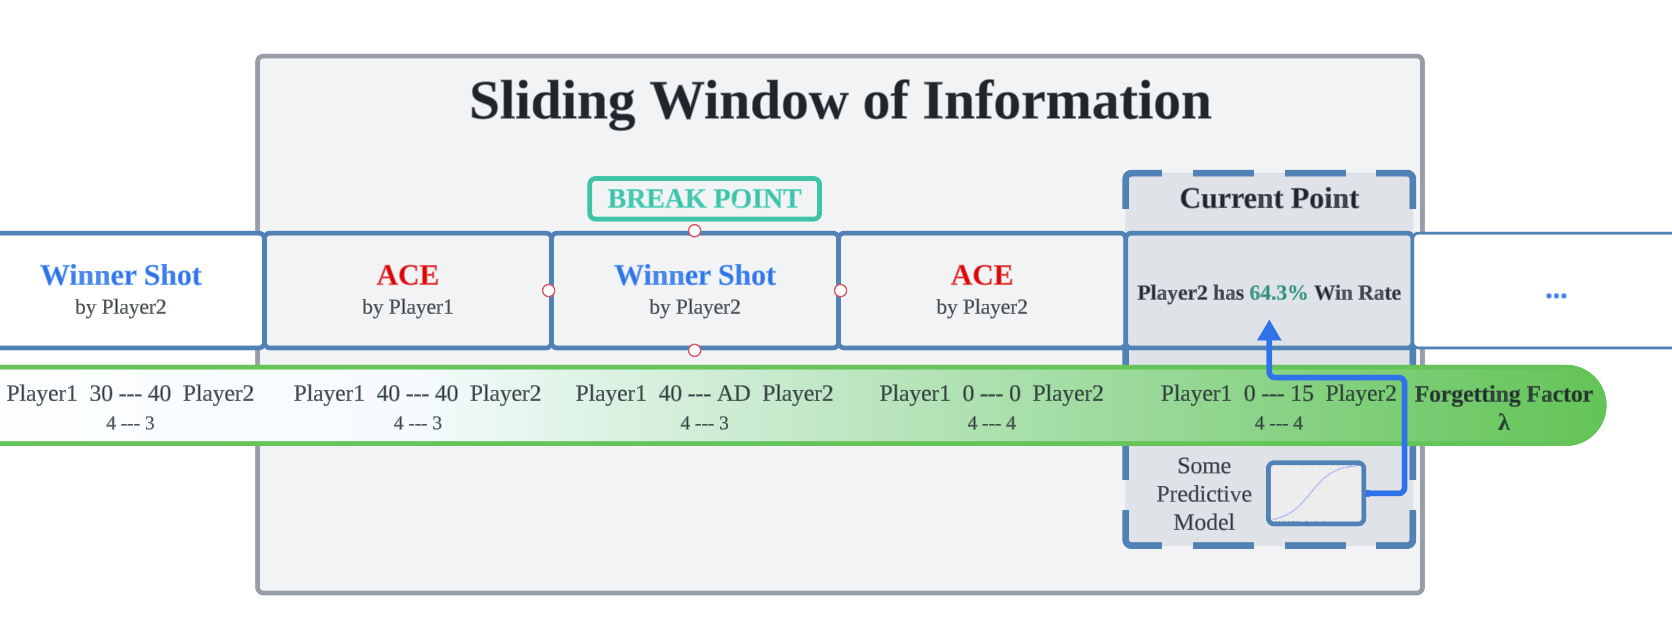
\includegraphics[width=.85\textwidth]{sliding-window.png} %图片的名称或者路径之中有空格会出问题 
	\caption{\centering Information Is Constrained by Sliding Window and Forgetting Factor. (Note that the data in this graph is for understanding the process.)} % 图片标题 
\end{figure}

\subsection{How to Describe Momentum and What Affects It}
To build an effective model that can analyze the player's momentum, we must first understand what "momentum" actually means. When we talk about momentum in tennis or any competitive sports, we are painting a picture of a player hitting their stride at just the right moment. The crowd can sense it, their cheers growing louder and more fervent. The players can feel it, their steps lighter, their spirits higher. 

\textit{However}, no matter how you would argue, "momentum" stays an elusive and subjective concept and largely a psychological state \cite{-1}; therefore, it is extremely hard to use an completely accurate numerical measurement for it, especially when we do not have available psychological data for these matches. With no measurement method, it is impossible to build a mathematical framework that could analyze the factors affecting the momentum, let alone predicting shifts in momentum as the match is being played. Worse yet, the momentum effect in tennis is highly controversial itself and is influenced by a complex interplay of factors, some measurable and some intangible.

Nonetheless, we argue that there is still a possible way to measure and model momentum. For example, in the final match of Wimbledon 2023, from when Djokovic won the first set with a dominating 6 to 1, to when Alcaraz took control in the third set with a same score but reversed for him, we can confidently say that there had been a shift in momentum. Therefore, while there is no established measurement of momentum, we can define a standard that momentum manifest itself in. In other words, we first designate a performance \textit{metric} that reflects momentum, such as the changes in scoring patterns, and then analyze how changes in this metric correlate with other observable factors and events during a match. This approach allows us to use quantitative data to infer the presence and impact of momentum, even if we cannot measure it directly. This process described in detail in the Figure :

\begin{figure}[htbp]  %h此处,t页顶,b页底,p独立一页,浮动体出现的位置
	\centering  %图表居中
	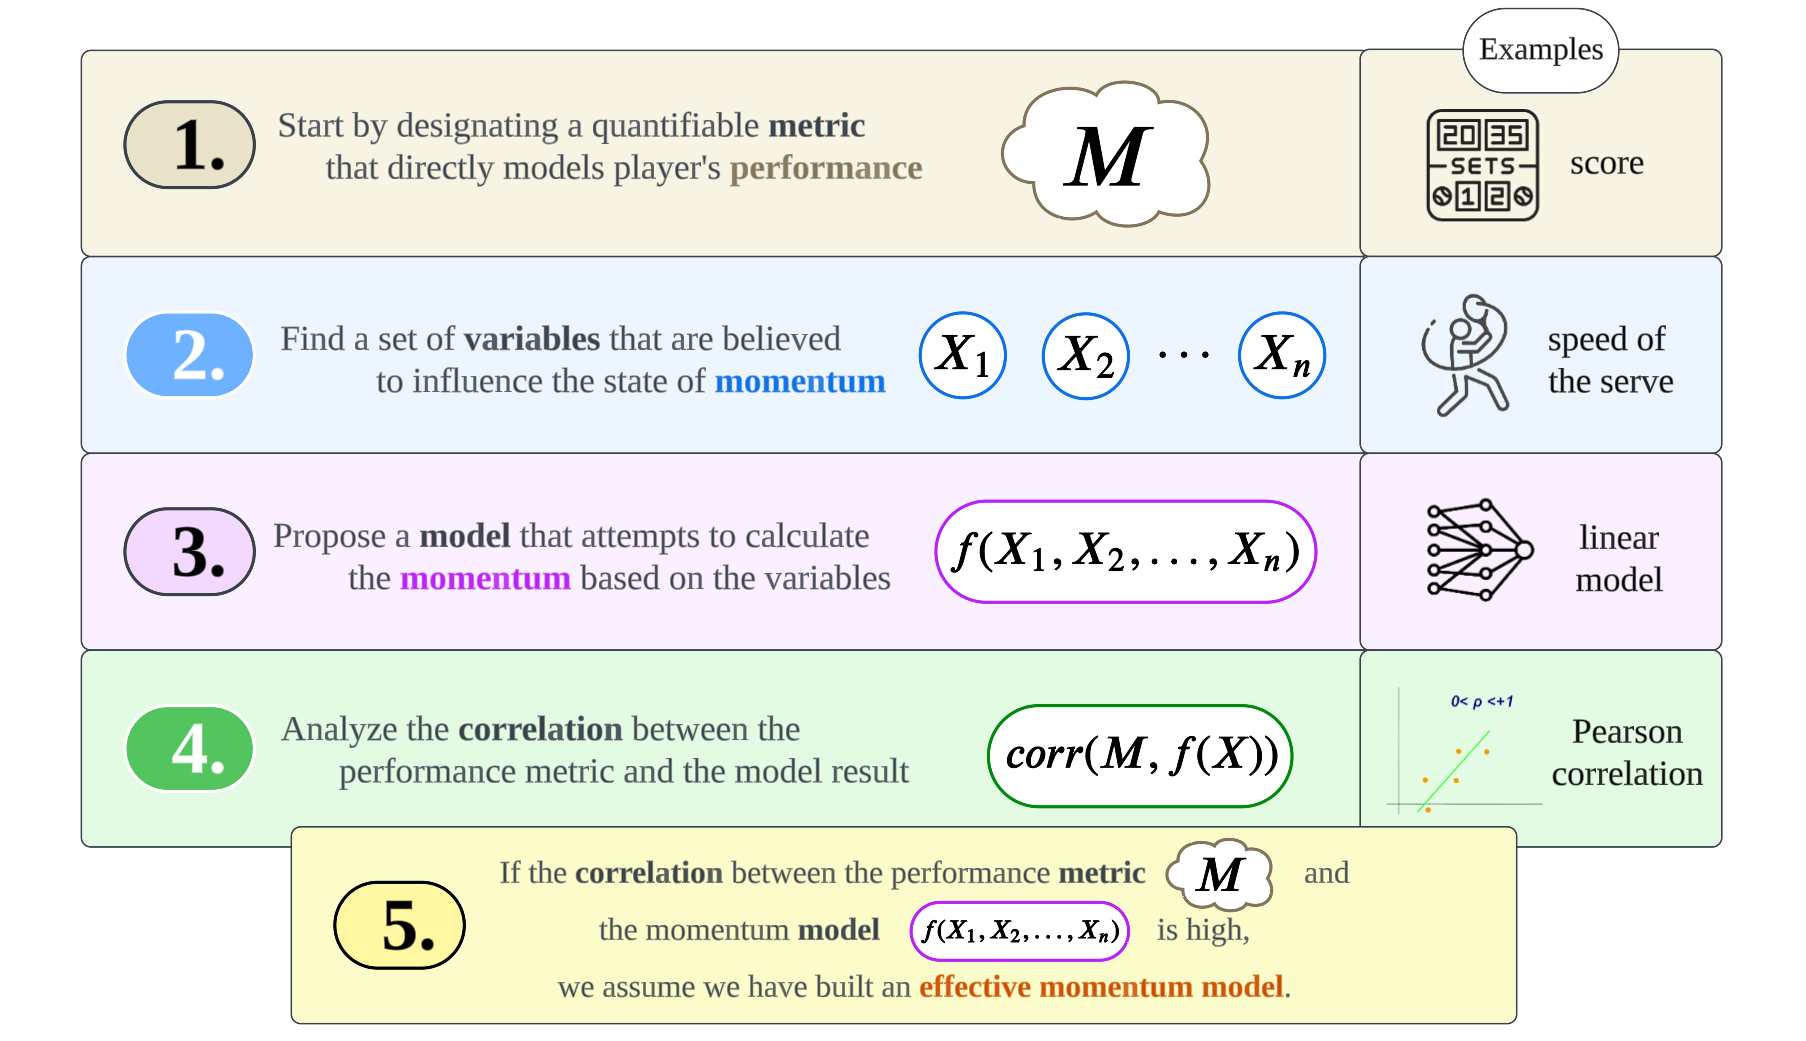
\includegraphics[width=\textwidth]{momentum-model.png} %图片的名称或者路径之中有空格会出问题 
	\caption{\centering Process of Modeling Momentum} % 图片标题 
\end{figure}

As described in the figure, if the correlation between the built momentum model and the performance metric are high, we can say that the momentum exists, affecting the ebb and flow during the match, and the model that attempts to calculate the momentum has a good credibility. The remaining work to do is to find the suitable parameters for the performance metric and look for factors to be incorporated into the momentum model, perhaps also leveraging the work of our first model that predicts the outcome of points. We note that any model of momentum, especially models that rely on physical match data, has a degree of uncertainty. We seek to capture the probability of shifts of games with our momentum model rather than deterministic outcomes.

If this method proves feasible in quantifying momentum, then other problems, such as predicting momentum shifts and utilizing the model to predict other matches, can be a straightforward process. If not, we will also identify the problems with our model and set a foundation for improving the model.

\subsection{Our Work}
It is our belief that a practical and inclusive mathematical framework to model the concept momentum would greatly help the tennis community in understanding the concept of momentum to improve performance, strategy, and training methodologies. In this paper, we seek to address this challenge using a set of match data from Wimbledon 2023 Men's Matches. Through extensive investigation in the field of tennis and thorough exploration, our main model - the \textbf{Momentum Quantifier (MoQ)}, integrates a comprehensive set of features and use a variety of statistical methods to achieve this goal. The building of this model can be overall described as follows:
\begin{enumerate}[\bfseries (1)]
	\setlength{\parsep}{0ex} %段落间距
	\setlength{\topsep}{2ex} %列表到上下文的垂直距离
	\setlength{\itemsep}{1ex} %条目间距
	\item To capture the flow of match in real-time, we constructed the CourtSense model as a sub-model of DTMA. The model starts by applying a Sliding Window machanism to a set of extracted features; these features are passed into the core Progressive Logisic Model that use the set of principal factors to predict the winning chance of the point; due to the real-time progression of the competition, a Forgetting Factor is added to dynamically update this model to reflect the most recent match status. 
	\item The mixture of the two drones is given and the extreme fire events is considered;
	\item Based on the verification model simulated by Poisson process and the hovering model based on Tabu Search, this article effectively demonstrates the validity and applicability.
\end{enumerate}
In order to avoid complicated description, intuitively reflect our work process, the flow chart is shown in Figure 3:

\begin{figure}[htbp]  %h此处,t页顶,b页底,p独立一页,浮动体出现的位置
	\centering  %图表居中
	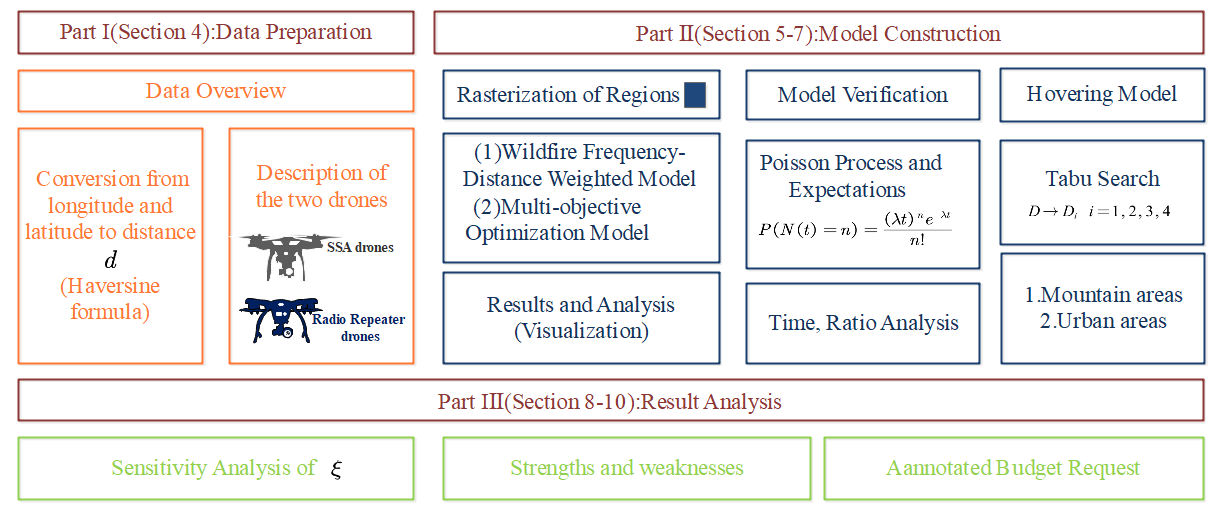
\includegraphics[width=.9\textwidth]{Flow_Chart.png} %图片的名称或者路径之中有空格会出问题 
	\caption{Flow Chart of Our Work} % 图片标题 
\end{figure}
\vspace{-0.8cm}


% 2. Assumptions 

\section{Model Preliminaries}
Considering that practical problems always contain many complex factors, first of all, we need to make reasonable assumptions to simplify the model, and each hypothesis is closely followed by its corresponding explanation:

\subsection{Assumptions}
\begin{enumerate}[\bfseries \textit{Assumption} 1:]
	\item \textbf{Only the influence of terrain on the drone is considered, and other factors such as temperature, humidity, and atmosphere are ignored.}\\
	\textbf{\textit{Explanation: }}The UAV's radiation communication range is only affected by terrain factors, and other factors are minimal. In fact, these factors affect each other, but in order to simplify the model ,we ignore the interactions between these factors.
	\item \textbf{The location of the EOC can be deployed around the fire due to an emergency.}\\
	\textbf{\textit{Explanation: }}The position of the EOC is not clearly given in the question. So, we assume that EOC can be set in a fire-free area around the wildfire site, since the glossary of the problem said that mobile EOC can be deployed near the site of an emergency.
	\item \textbf{The "boots-on-the-ground" forward teams can be approximated as near the fire site.}\\
	\textbf{\textit{Explanation: }}The actual movement of the team is very complicated, and it is difficult to accurately calculate its position. Therefore, it is assumed that the squad is near the fire field and the drone arrives at the fire field to establish a connection with the squad.
	\item \textbf{The collected data can be considered reliable and can reflect the changing laws of the Victorian wildfire.}\\
	\textbf{\textit{Explanation: }}The historical Victorian wildfire data, latitude, longitude and other data come from authoritative websites, such as the official website of FEC in Australia and NASA, with high accuracy.
\end{enumerate}
Additional assumptions are made to simplify analysis for individual sections. These assumptions will be discussed at the appropriate locations.




% 3. Notation

\subsection{Notations}
Some important mathematical notations used in this paper are listed in Table 1. 
\begin{table}[htbp]
\begin{center}
\caption{Notations used in this paper}
\begin{tabular}{c l}
\toprule[2pt]
\multicolumn{1}{m{3cm}}{\centering Symbol} & \multicolumn{1}{m{8cm}}{\centering Description }\\
\midrule
$x_i$ & Longitude within the i-th Wildfire Grid \\
$y_i$ & Latitude within the i-th Wildfire Grid \\
$\varOmega _i$ & The area of the i-th grid\\
$d_{ki}$ & the distance $d_{ki}$ between the k-th roaming grid and the i-th grid \\
$SC_k$ & Score for evaluating the k-th wildfire grid \\
\vspace{5pt}%公式间有点挤,空一些
$x^{( \alpha )}_{ki}$ & the $SSA_\alpha$ drone sent by the k-th EOC to the i-th wild-fire grid\\
\vspace{3pt}
$x^{( \beta )}_{ki}$ & the $RR_\beta$ drone sent by the k-th EOC to the i-th wildfire grid\\
$t_{fly}^{\delta}$ & The flight time of drones\\
\bottomrule[2pt]
\end{tabular}\label{tb:notation}
 \begin{tablenotes}
        \footnotesize
        \item[*] *There are some variables that are not listed here and will be discussed in detail in each section. %此处加入注释*信息
      \end{tablenotes}
\end{center}
\end{table}
\vspace{-1cm}%在\end{table}下加一行\vspace{-1cm} 其中-1的作用是缩短与下方文字距离的 切记!必须是负数





% 4. Model

\section{CourtSense: Understanding the State of Match}
The CourtSense model aims to capture the current state of the match by predicting the outcome of the next unplayed point, using available match information. First, we need to apply feature engineering to the given data to extract useful features.

\subsection{Feature Engineering}

\subsubsection{Data Extraction}
The data provided by the problem (\textit{Wimbledon\_featured\_matches.csv}) is a comprehensive dataset that contains the complete match information, including scores, serve details, point details which are all applicable to analyze the state of the match. After a thorough inspection of the data, we find that the data is clean and usable. However, these are all explicit match information and is limited to a specific point, for example, whether this player is serving, what is the ratio of scores, etc. We think that more temporal features like whether this player is leading in score are more direct in describing the match’s status; hence we added them to the feature set. These additional features are included in Table 2.


\begin{table}[htbp]
	\centering  % Use \centering instead of the center environment to avoid extra vertical space
	\caption{Added Match Information}
	\resizebox{\textwidth}{!}{% Adjusted the resizebox command
		\begin{tabular}{ccc}  % Simplified column specification since you're centering all cells
			\toprule[2pt]
			\multicolumn{1}{m{4cm}}{\centering \textbf{Column Name}} &
			\multicolumn{1}{m{8cm}}{\centering \textbf{Description}} & 
		\multicolumn{1}{m{5cm}}{\centering \textbf{Example Value}} \\ 
	\midrule
	p1\_streak & The winning / losing streak of player 1 up until that point & 5, 0, -3 \\
	p2\_streak & The winning / losing streak of player 2 up until that point & 3, 0, -5 \\ 
	p1\_leading & Whether p1 is leading in score & 1 (leading), 0, -1 \\
	p2\_leading & Whether p1 is leading in score & -1 (losing), 0, 1 \\
	p1\_leading\_game & Whether p1 is leading in game & 1, 0, -1 \\
	p2\_leading\_game & Whether p1 is leading in game & -1, 0, 1 \\
	p1\_leading\_set & Whether p1 is leading in set & 1, 0, -1 \\
	p2\_leading\_set & Whether p1 is leading in set & -1, 0, 1 \\
	\bottomrule[2pt]
\end{tabular}
}
\end{table}

These features, representing nuanced indicators of the current state of the match, are better to feed into the model than raw scores for simplicity and accuracy. For example, the winning streak is a direct reflection of the player's current performance and momentum.

Moreover, for the data columns like '\textit{game\_victor}' that represent the winner of the game (or set), we split them into 2 columns to be player-specific. For each point \( i \) in the match, we transform, for example, the \textit{game\_victor} column into two player-specific columns, \( V_{p1}^{(i)} \) and \( V_{p2}^{(i)} \), defined as:
\[
V_{p1}^{(i)} = 
\begin{cases} 
	1 & \text{if \textit{game\_victor} = 1 at point } i  \\
	-1 & \text{if \textit{game\_victor} = 2 at point } i \\
	0 & \text{if if \textit{game\_victor} = 0 at point } i
\end{cases}
\]

\[
V_{p2}^{(i)} = 
\begin{cases} 
	1 & \text{if \textit{game\_victor} = 2 at point } i \\
	-1 & \text{if \textit{game\_victor} = 1 at point } i \\
	0 & \text{if if \textit{game\_victor} = 0 at point } i
\end{cases}
\]
this procedure ensures these data can be modeled as their respective performance.  

Finally, we discarded other rather unimportant or redundant information for the match, such as the raw score information, the speed of the serve (which cannot be used for points already in play when predicting point outcomes), unforced errors (less indicative of player's performance), and information about net points. These choices are made after conducting a thorough research on related Sports Analytics in the field of tennis \cite{2}\cite{3}\cite{4}. The remaining features alongside the constructed features can be used as raw input data for our model.

\subsubsection{Sliding Window Mechanism}
We recognize that the current state of the match is heavily influenced by the temporal features of, not only for the current point, but also the last few points. For example, if the player ran a long distance in the past few point rounds, they will carry more amount of fatigue, influencing the player's performance of the current point. Or if the player has just won a break point, they will gain much more confidence in their coming plays. Therefore, by employing a sliding window mechanism, the model can utilize the temporal features on the most recent and relevant data points, ensuring that the analysis remains sensitive to the current state of play and the immediate history before it. This is described in the formula below:

Let \( F_{t} \) and \( F_{nt} \) represent the sets of temporal and non-temporal features, respectively. For a given point in time \( t \), the combined feature set \( F^{(t)} \) is given by:

\[
F^{(t)} = S_{t}^{(t-1)} \cup F_{nt}^{(t)}
\]
where

\[
S_{t}^{(t-1)} = \sum_{i=t-3}^{t-1} F_{t}^{(i)}
\]
represents the sum of temporal features of last 3 points played, and \( F_{nt} \) represents the non-temporal features at the current point \( t \). The temporal features include whether the player just had a break point, or double fault, etc., which could affect the performance of the current play; the non-temporal features include whether this player is serving at this point, and the winning streak, etc.

So far, we have acquired a granular and exhaustive set features that completely describe the match's status at a specific point and is ready to be fed into our Progressive Logistic Model - the core of the CourtSense model.

\subsection{Progressive Logistic Model}
To effectively capture the dynamic flow of a tennis match, we introduce the Progressive Logistic Model. This model is designed to predict the outcome probability of the current point, providing a real-time assessment of the match's status and the relative performances of the players. The Progressive Logistic Model utilizes a multivariate logistic regression framework, due to its suitability for binary outcome prediction (e.g., point won or lost) and its ability to output probabilities based on multiple features; furthermore, combined with the Forgetting Factor, the model is capable of progressively updating the itself according to the latest match information as the match progresses. The general process of this model is depicted in Figure 3. 

\begin{figure}[htbp]  %h此处,t页顶,b页底,p独立一页,浮动体出现的位置
	\centering  %图表居中
	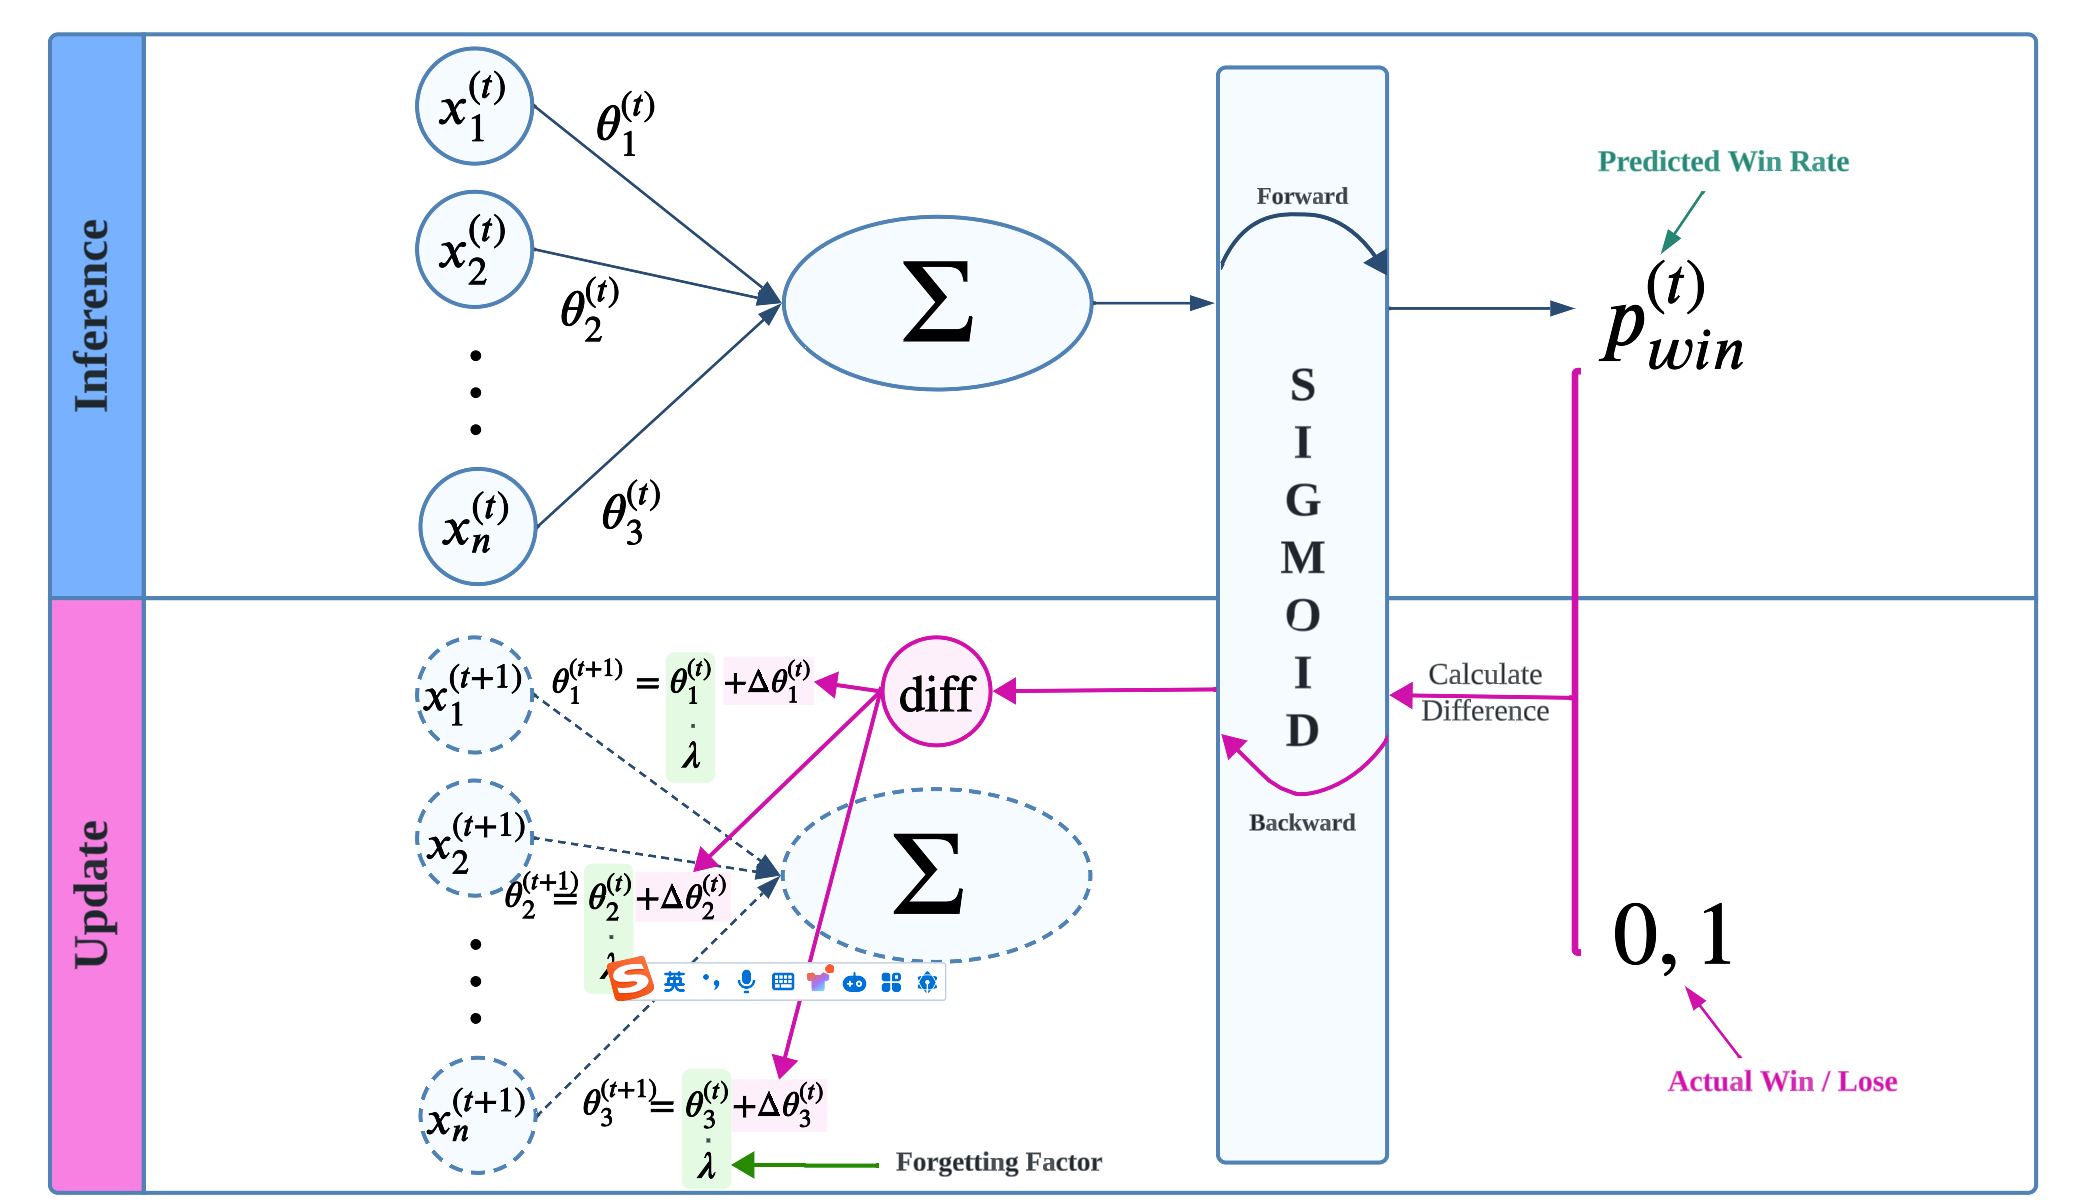
\includegraphics[width=.9\textwidth]{logistic.png} %图片的名称或者路径之中有空格会出问题 
	\caption{Process of the Progressive Logistic Regression Model} % 图片标题 
\end{figure}
\vspace{-0.8cm}

\subsubsection{Model Establishment}
Logistic regression is a statistical model used for binary classification problems, developed by David Cox in 1958. It is a type of generalized linear model (GLM) that uses a logistic function to model a binary dependent variable. The goal of logistic regression is to find the best fitting model to describe the relationship between the dichotomous characteristic of interest (dependent variable = 0 or 1) and a set of independent variables (predictors) \cite{5}. While the assumption of variable independence is ideal, logistic regression can still perform effectively in real-world scenarios where complete independence is rare, such as our feature set that describe match's information.

To feed the aggregated features into a logistic regression model, each feature set is represented as a vector $\mathbf{x}^{(t)}$ at timestep t (which means the t-th point played in this match), and these vectors are used to calculate the probability of winning a point. $\mathbf{x}^{(t)}$ is directly derived from the feature set \( F^{(t)} \), which contains both temporal features and non-temporal features.

The logistic regression model predicts the probability $ P(y^{(t)}=1|\mathbf{x}^{(t)}; \mathbf{\theta}) $
where $y^{(t)}=1$ indicates the event of interest (i.e., winning the point), $x^{(t)}$ is the feature vector at timestep $t$, and $\mathbf{\theta}$ represents the model parameter (weights). The model calculates the probability using the formula below:
\[
P(y^{(t)}=1|\mathbf{x}^{(t)}; \mathbf{\theta}) = \sigma(\mathbf{\theta}^\top \mathbf{x}^{(t)})
\]
where \( \sigma(z) \) is the sigmoid function defined as:
\[
\sigma(z) = \frac{1}{1 + e^{-z}}
\]
and \( z = \mathbf{\theta}^\top \mathbf{x}^{(t)} \) represents the linear combination of the features \( \mathbf{x}^{(t)} \) weighted by the model parameters \( \mathbf{\theta} \), expressed as:
\[
z = \theta_0 + \theta_1 x_1^{(t)} + \theta_2 x_2^{(t)} + \cdots + \theta_n x_n^{(t)}
\]
where \( \theta_0 \) is the intercept term, \( \theta_1, \theta_2, \ldots, \theta_n \) are the weights associated with each feature \( x_1^{(t)}, x_2^{(t)}, \ldots, x_n^{(t)} \) in the feature vector \( \mathbf{x}^{(t)} \).

Once we have the correct set of model parameters, we can determine the winning probability of a player based on the feature vector of the match for that player.


\subsubsection{Parameters Training \& Updating}
One of our Progressive Logistic Model's highlights is its ability to progressively adjust itself during the play of the match. But this does not mean it relies only on the real-time data; instead, we first train the model using the data given by the problem (pre-training phase), and when applied to a specific match, the progressive real-time data updates the parameters as the match unfolds (updating phase).

The training of the logistic regression model's parameters $\mathbf{\theta}$ is achieved by minimizing the logistic loss function, which quantifies the difference between the predicted outcomes and the actual results of matches:
\[
\mathcal{L}(\mathbf{\theta}) = -\frac{1}{m} \sum_{i=1}^{m} \left[ y^{(i)} \log(\sigma(\mathbf{\theta}^\top \mathbf{x}^{(i)})) + (1 - y^{(i)}) \log(1 - \sigma(\mathbf{\theta}^\top \mathbf{x}^{(i)})) \right]
\]
where \( m \) represents the number of observations in the training dataset, \( y^{(i)} \) denotes the outcome of the \( i \)-th point (win or loss), and \( \mathbf{x}^{(i)} \) is the feature vector associated with the \( i \)-th point in a match. Then, the parameter vector \( \mathbf{\theta} \) is optimized performed using Gradient Descent, described as:
\[
\mathbf{\theta} := \mathbf{\theta} - \alpha \nabla_{\mathbf{\theta}} \mathcal{L}(\mathbf{\theta})
\]
where \( \alpha \) is the learning rate that regulates the step size during each iteration, and \( \nabla_{\mathbf{\theta}} \mathcal{L}(\mathbf{\theta}) \) represents the gradient of the loss function with respect to the parameter vector \( \mathbf{\theta} \). Considering the constraints of the size of the dataset and the model's ability to update itself during a match, we meticulously choose different values for pre-training our model and updating our model during the match:
\[
\alpha = 
\begin{cases} 
	0.01 & \text{at pre-training phase } \\
	0.05 & \text{at updating phase } 
\end{cases}
\]
in this way, for each data point, both when pre-training and when updating, the parameter vector is iteratively updated in the direction that reduces the loss function.

At updating phase, the logistic regression model's parameters (\( \mathbf{\theta} \)) need to reflect the latest match data. This requires us to place more weight to the latest information of the points. Therefore, aside from using a higher learning rate value, a forgetting factor \( \lambda \) is incorporated into the parameter update rule:

\[
\mathbf{\theta}^{(t)} = \lambda \cdot \mathbf{\theta}^{(t-1)} +  \Delta\mathbf{\theta}^{(t-1)}
\]
\[ 
\Delta\mathbf{\theta}^{(t-1)} = - (1 - \lambda) \alpha \nabla_{\mathbf{\theta}^{(t-1)}} \mathcal{L}(\mathbf{\theta}^{(t-1)})
\]
this rule adjusts $\mathbf{\theta}^{(t)}$ by blending the previous parameters  \( \mathbf{\theta}^{(t-1)} \), scaled by \( \lambda \), with the changes updated by new data (\( - \alpha \nabla_{\mathbf{\theta}^{(t-1)}} \mathcal{L}(\mathbf{\theta}^{(t-1)}) \)), scaled by $ (1 - \lambda) $. In such a way, the forgetting factor allows the model to prioritize recent information and adapt to changes in gameplay strategies or player performance over time.

To this point, we have thoroughly established our CourtSense model, which first uses feature selection combined with a sliding window mechanism, and leverages a Progressive Logistic Model to follow the flow of the match and predict the result of a specific point. 

The original dataset of \textit{Wimbledon\_featured\_matches.csv} included the matches played at Wimbledon 2023 from the 3rd round to the final round (7th round), with a total of 7256 points. To separate the training and testing sets, we use the data of the 30 matches from the 3rd round to the semi-final round (a total of 6950 points), and use the epic match in the final round (334 points) between Carlos Alcaraz and Novak Djokovic to test our model's accuracy.

We train our CourtSense model using Scikit-learn, a machine learning framework for Python. After pre-training, the CourtSense Model is then tested on the testing set, where the model starts from predicting the winning probabilities of both players at the first point, and updates itself based the actual result of the first point, and then moves on to predict the second point, etc. The aggregated results of all point predictions and their actual outcomes are used for validating our model's performance.

\subsection{Model Validation}

In validating the performance of our CourtSense model, we focused on a suite of standard evaluation metrics, including Mean Squared Error (MSE), accuracy, confusion matrix, and AUC-ROC. MSE represents how far the model's predictions are from the actual values; accuracy measures the proportion of total predictions our model gets right; the confusion matrix shows exactly how many values were predicted correctly or falsely; AUC provides an insight into the model's ability to distinguish between the two possible outcomes (winning or losing a point), with higher values close to 1 indicating better performance. The detailed explanation can be found in \cite{6}. The result of these metrics are shown in Table 3 and Figure 7.
\begin{table}[htbp]
	\centering
	\caption{Evaluation Metrics Result for CourtSense Model}
	\resizebox{0.7\textwidth}{!}{% Ensure this scales the table appropriately
		\begin{tabular}{ccc} % You can use 'c' alignment since you're centering all cells
			\toprule[2pt]
			\multicolumn{1}{m{4cm}}{\centering \textbf{Metric}} &
			\multicolumn{1}{m{4cm}}{\centering \textbf{Value for Player 1}} &
			\multicolumn{1}{m{4cm}}{\centering \textbf{Value for Player 2}} \\
			\midrule
			MSE & 19.57\% & 19.02\% \\
			Accuracy & 92.52\% & 93.11\% \\
			AUC-ROC & 93.886\% & 93.445\% \\
			\bottomrule[2pt]
		\end{tabular}
	}
\end{table}
\vspace{0.8cm}
\begin{figure}[htbp]  %h此处,t页顶,b页底,p独立一页,浮动体出现的位置
	\centering  %图表居中
	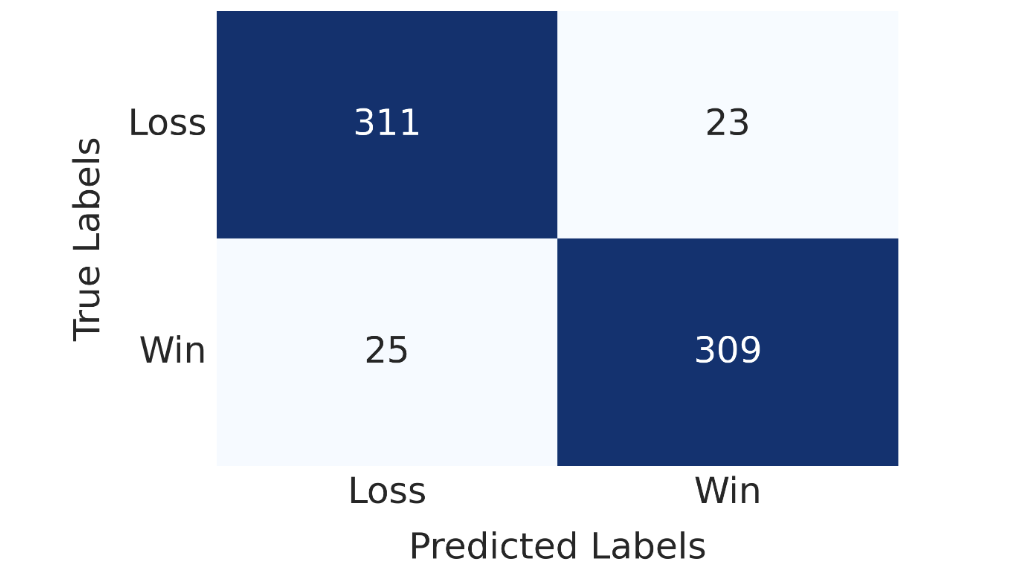
\includegraphics[width=.5\textwidth]{confusion-matrix.png} %图片的名称或者路径之中有空格会出问题 
	\caption{Confusion Matrix for CourtSense Model} % 图片标题 
\end{figure}
\vspace{-0.8cm}

To our surprise, the CourtSense model performs exceedingly well at predicting each point's outcome during the match. It is almost too good: the model achieved an average accuracy of 92.82\%, while the AUC stood at an average of 93.67\%, suggesting that the model can reliably forecast match dynamics, providing valuable insights into players' performance. This could be attributed to our meticulous selection of features and the various mechanisms our model used.

In addition to evaluating the overall performance of our CourtSense model, we also analyzed on its adaptability throughout the progression of a match. We analyzed the model's accuracy in predicting outcomes by computing a moving average across 20-point windows. This approach allowed us to observe how the model's predictive accuracy fluctuated over the course of a match. The resulting data is illustrated in Figure 8. 

\begin{figure}[htbp]  %h此处,t页顶,b页底,p独立一页,浮动体出现的位置
	\centering  %图表居中
	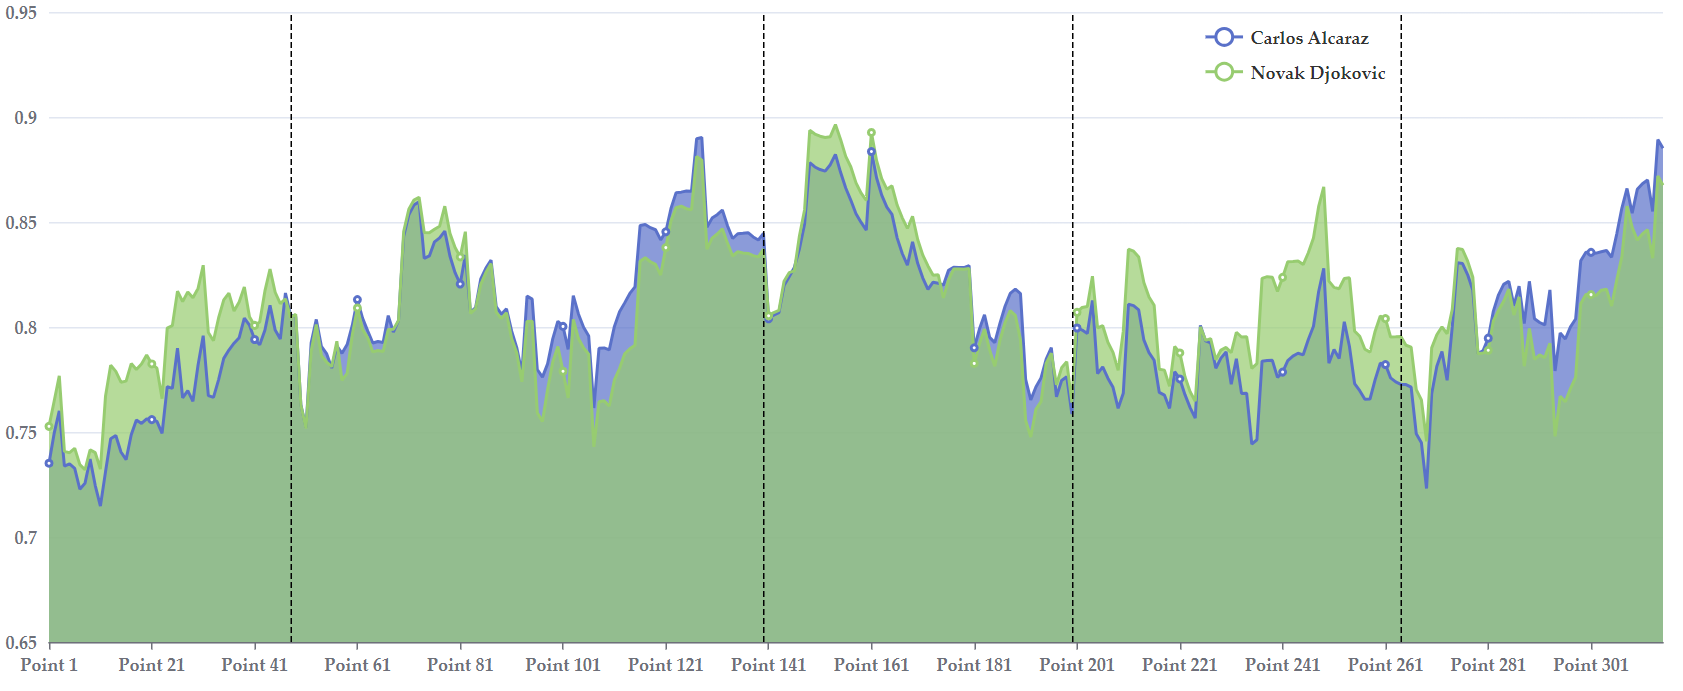
\includegraphics[width=.8\textwidth]{moving-average.png} %图片的名称或者路径之中有空格会出问题 
	\caption{Average Predictive Power of CourtSense as Match Unfolds} % 图片标题 
\end{figure}
\vspace{-0.2cm}

We can see the model starts at a relatively low accuracy, and moves up as the match unfolds. Generally, for each set of the game (as separated by the vertical lines in the graph), the model is able to progressively adapt its parameters to better fit the match's status, although there are some fluctuations, probably signaling a randomness for the outcome of the points.

\subsection{Match Flow Visualization}
To visualize the flow of the match, we select the 2nd set of the final match between Carlos Alcaraz and Novak Djokovic, which was an intense play with a tie-breaker of 7-6. Figure 9 presents a graphical depiction of the prediction difference between the two players, which indicates their performance differences, over the course of this set. The vertical axis is the difference in the predicted probability of winning each point; while the horizontal axis represents the sequence of points played. When the curve rises above the zero line, it suggests that Player 1 is more likely to win the point; when it dips below, Player 2 is favored. The dotted line at 0.08 reflects the average prediction difference across all points, which is a little above 0 (happens to reflect the tie-breaker win of Alcaraz).

\begin{figure}[htbp]  %h此处,t页顶,b页底,p独立一页,浮动体出现的位置
	\centering  %图表居中
	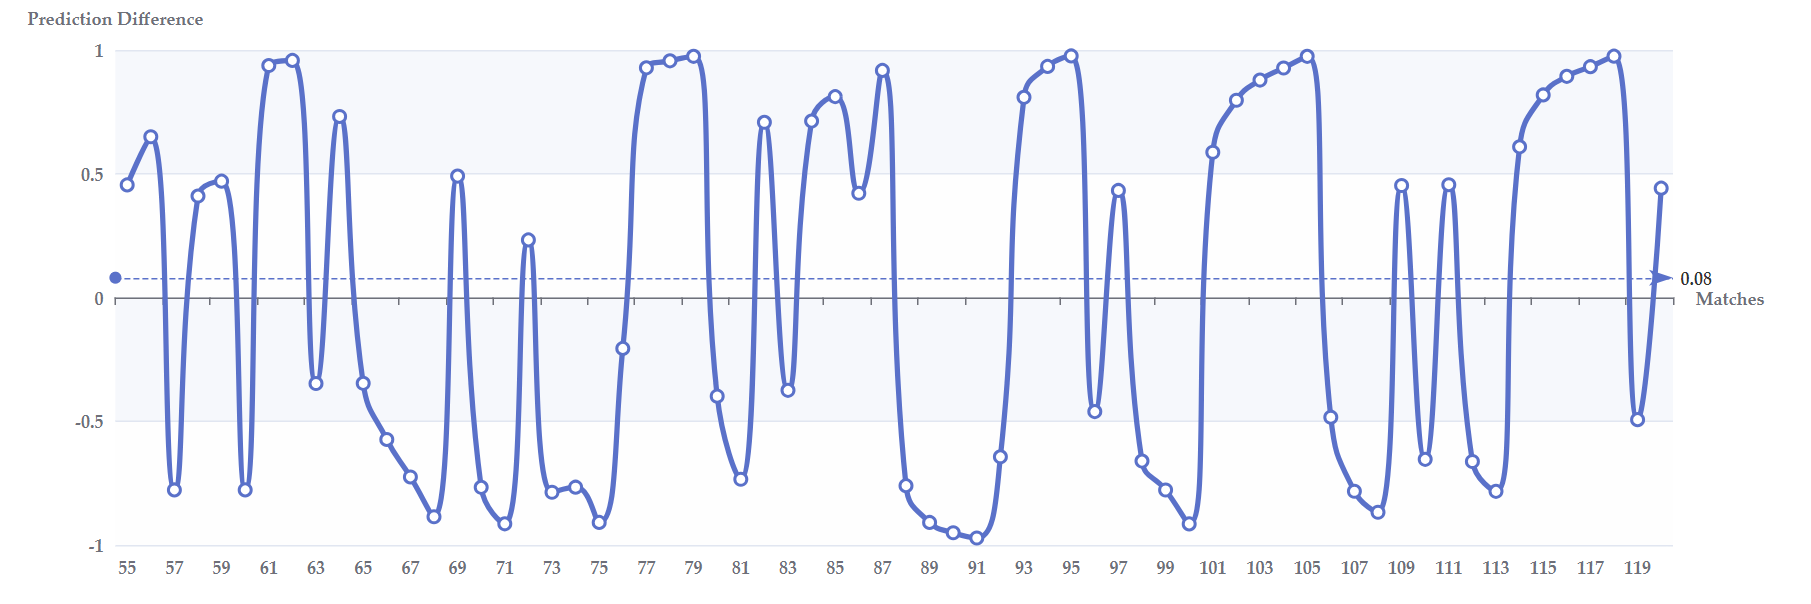
\includegraphics[width=.8\textwidth]{prediction-difference.png} %图片的名称或者路径之中有空格会出问题 
	\caption{Match's Flow during the 2nd Set of the Final Match, Indicated by the Winning Chance Difference} % 图片标题 
\end{figure}
%\vspace{-0.8cm}

The fluctuations in the graph traces the ebb and flow of the match, or perhaps, the real-time shifts in "momentum" between the players during the match. These shifts are marked by rapid ascents and descents in the curve. Notably, a player often maintains this momentum for a sequence of points before it changes to the other player, illustrating the competitive nature of a tennis match. But does the graph capture a true flow of "momentum", or is it merely an illusion of temporary advantage? We'll discuss this problem by advancing our model below.

\section{Momentum Quantifier (MoQ): Decoding the Myth of Momentum}

As discussed in the Problem Analysis section, we think that momentum is an elusive concept and cannot be measured directly; but it can be reflected by the changing patterns of score. By defining a performance metric like this, we can try to develop a model (Momentum Quantifier, MoQ) that calculates the amount of momentum based a set of anticipated factors, and if the MoQ's result has high correlation value with the metric, we are safe to say the model is effective for analyzing and quantifying momentum. 

\subsection{Designating a Performance Metric}
This brings back to the question: does the chance of winning a specific point reflect the momentum? While the granular details of every point matter, we think that momentum is more about the \textit{broader strokes} of the match — the ebb and flow felt over games and sets. So although predicting each point's outcome can be influential, we also need to consider \textbf{a suitable scope of} score that can reflect the volume of momentum. Under this scope, we calculate gained-score differences. For example, during the the 5th set between Alcaraz and Djokovic, their difference between their gained points in a scope of 12 points, are depicted as below in Figure: 

\begin{figure}[htbp]  %h此处,t页顶,b页底,p独立一页,浮动体出现的位置
	\centering  %图表居中
	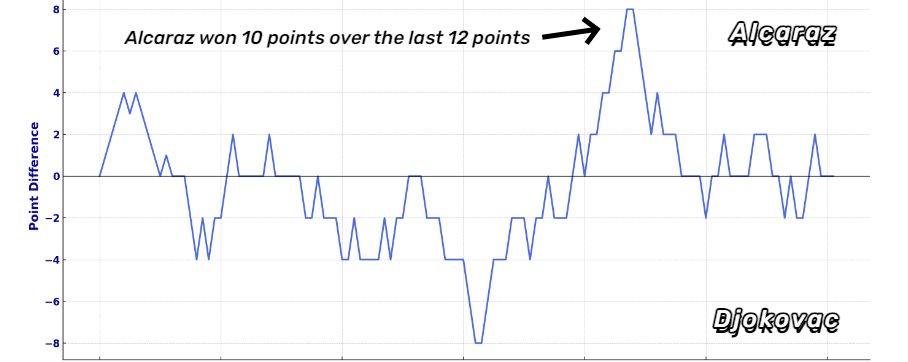
\includegraphics[width=.6\textwidth]{difference.png} %图片的名称或者路径之中有空格会出问题 
	\caption{Sum of gained point differences within a scope of 12 points} % 图片标题 
\end{figure}
\vspace{-0.2cm}

We can clearly see that at the middle point in the match, Djokovic has a significant edge over Alcaraz at first, before Alcaraz taking back the momentum and chased the points back by winning 10 points in the last 12 points. The actual flow of momentum, as we watched the match from \cite{7} and inferred from the live atmosphere, is quite similar with the flow of this graph. This means this the scoped gained-score difference is indeed a performance metric good at reflecting momentum.

We designated our performance metric as the following. Denote the set of points won by player \( A \) in a given scope as \( P_A \), and \( P_B \) for player \( B \), with the scope defined as the last \( N \) points played. The performance metric, \( M \), for player \( A \) over player \( B \) in this scope can then be defined as:
\[
M=\sum_{i=1}^{N}(P_{A}^i-P_{B}^i)
\]
where \( P_{A_i} \) and \( P_{B_i} \) are binary indicators of whether player \( A \) or \( B \) won the \( i^{th} \) point in the scope, respectively. Specifically, \( P_{A_i} = 1 \) if player \( A \) won the \( i^{th} \) point, and 0 otherwise; similarly for \( P_{B_i} \). After careful consideration and collection, we eventually chose a value of 12 for the scope $N$.

However, there is some nuance here. As discussed, our goal is to build a momentum model that incorporates some important factors at a \textit{specific point} to measure its momentum. Apparently, the gained-score difference within the scope N is an \textit{average} performance difference in that scope, not indicator of momentum of any specific point. For instance, if we look at the highest point in Figure , it means Alcaraz took the 8 points of the 12 points before the play of this point. This difference only signals he has played well in the last 12 points in general, not an performance indicator of the current point; and as we can see, this difference dropped sharply after this point, signaling the momentum is shifting towards his opponent at this point.

Reviewing our problem, we eventually aim to predict shifts in momentum as the match progresses. Therefore, when training our model, it would be rational to use the N points \textit{after} the point of concern rather than \textit{before} that point; in this way, the model is able to \textit{predict} the average momentum after that point. This choice is made after we found that, the model trained using scoped gained-score difference before that point achieved little correlation with this metric. Finally, the performance metric of point $t$ in the match is defined as:
\[
M^{(t)}=\sum_{i=t}^{t+N}(P_{A}^i-P_{B}^i)
\]

\subsection{Determining the Factors of Momentum}
Before defining the structure of the MoQ model, we first need to find the possible factors of momentum. After an extensive research in this field \cite{8} \cite{9}, we eventually defined the \textbf{4S} factors (Scoring, Serve, Stamina, and Slip) to account for factors that may affect the shifts in momentum:

\begin{enumerate}[\bfseries S1.]
	\item \textbf{Scoring Factor: point\_win}\\
	\textbf{\textit{Explanation: }}We use the result of our CourtSense model, which is capable predicting the outcome of the immediate point, as scoring factor. This will model how the chances of winning the current point affect the flow of momentum.
	\item \textbf{Service Factor: server, break\_pt\_won, ace}\\
	\textbf{\textit{Explanation: }}The statistics of serves heavily impacts the shift of momentum in tennis, especially when acing and winning a break point.
	\item \textbf{Stamina Factor: distance\_run, speed\_mph, rally\_count, serve\_depth, serve\_width, return\_depth}\\
	\textbf{\textit{Explanation: }}We believe these stamina factors that reflect the quality of the play are also influential in momentum.
	\item \textbf{Slip Factor: double\_fault, unf\_err}\\
	\textbf{\textit{Explanation: }}Small mistakes like unforced errors and double fault of a player, although not significant in actual performance, can potentially cause a psychological fluctuation, thereby affecting momentum. 
\end{enumerate}

\subsection{MoQ's Core: Time-Series Analysis with LSTM}
In this part, we describe the main model structure used in our MoQ model. Now that we have the factors that may affect the volume of momentum, we need to build a model that quantifies momentum and predict momentum shifts. Note the 4S factors are point-specific data, and points are essentially a time-series within a match:
\[ 
	S = \{s^{(1)}, s^{(2)}, ..., s^{(n)}\}
\]
where each element in series $S$ is a value such that $s^{(t)}={f(x_1^{(t)}, x_2^{(t)}, ..., x_m^{(t)})}$, with $x_1^{(t)}, x_2^{(t)}, ..., x_m^{(t)}$ being our 4S factors, the function $f$ defined by a specific model. Also, note the model's goal of forecast shifts in momentum. In this scenario, we think of using \textbf{multivariate time series} models in the field of machine learning \cite{10}. Finally, we choose the Long-Term Short Memory Recurrent Neural Network (LSTM), considering this model's capability of to handle multivariate series data \cite{11}.
\subsubsection{LSTM Structure}

The LSTM unit comprises three primary \textbf{gates}: the input gate, the forget gate, and the output gate, alongside two \textbf{states}: the cell state and the hidden state. To explain what these mean, imagine LSTM as a kind of smart agent that watches a sequence of events (momentum changes in a tennis match in our case) unfold over time. This agent has a special notebook (\textbf{the cell state}) where it can jot down important information to remember and also erase things that are no longer relevant. Alongside, it has a certain level of focus or attention (\textbf{the hidden state}) that it adjusts based on the latest events and what it has decided to keep in its notebook. These decisions are made by three specialized mechanisms, often referred to as gates. \textbf{The Forget Gate} decides what from its notebook is no longer useful and can be erased. It looks at the new information and the current state of focus and decides what memories to let go of. \textbf{The Input Gate} helps the agent decide which of the \textit{new} information is important enough to note down in its notebook. After updating its notebook and deciding what to focus on, \textbf{the Output Gate} uses this gate to determine what it should pay attention to now. This is based on its updated notebook and the new information, guiding its current state of focus or attention. This process is illustrated in Figure .

\begin{figure}[htbp]  %h此处,t页顶,b页底,p独立一页,浮动体出现的位置
	\centering  %图表居中
	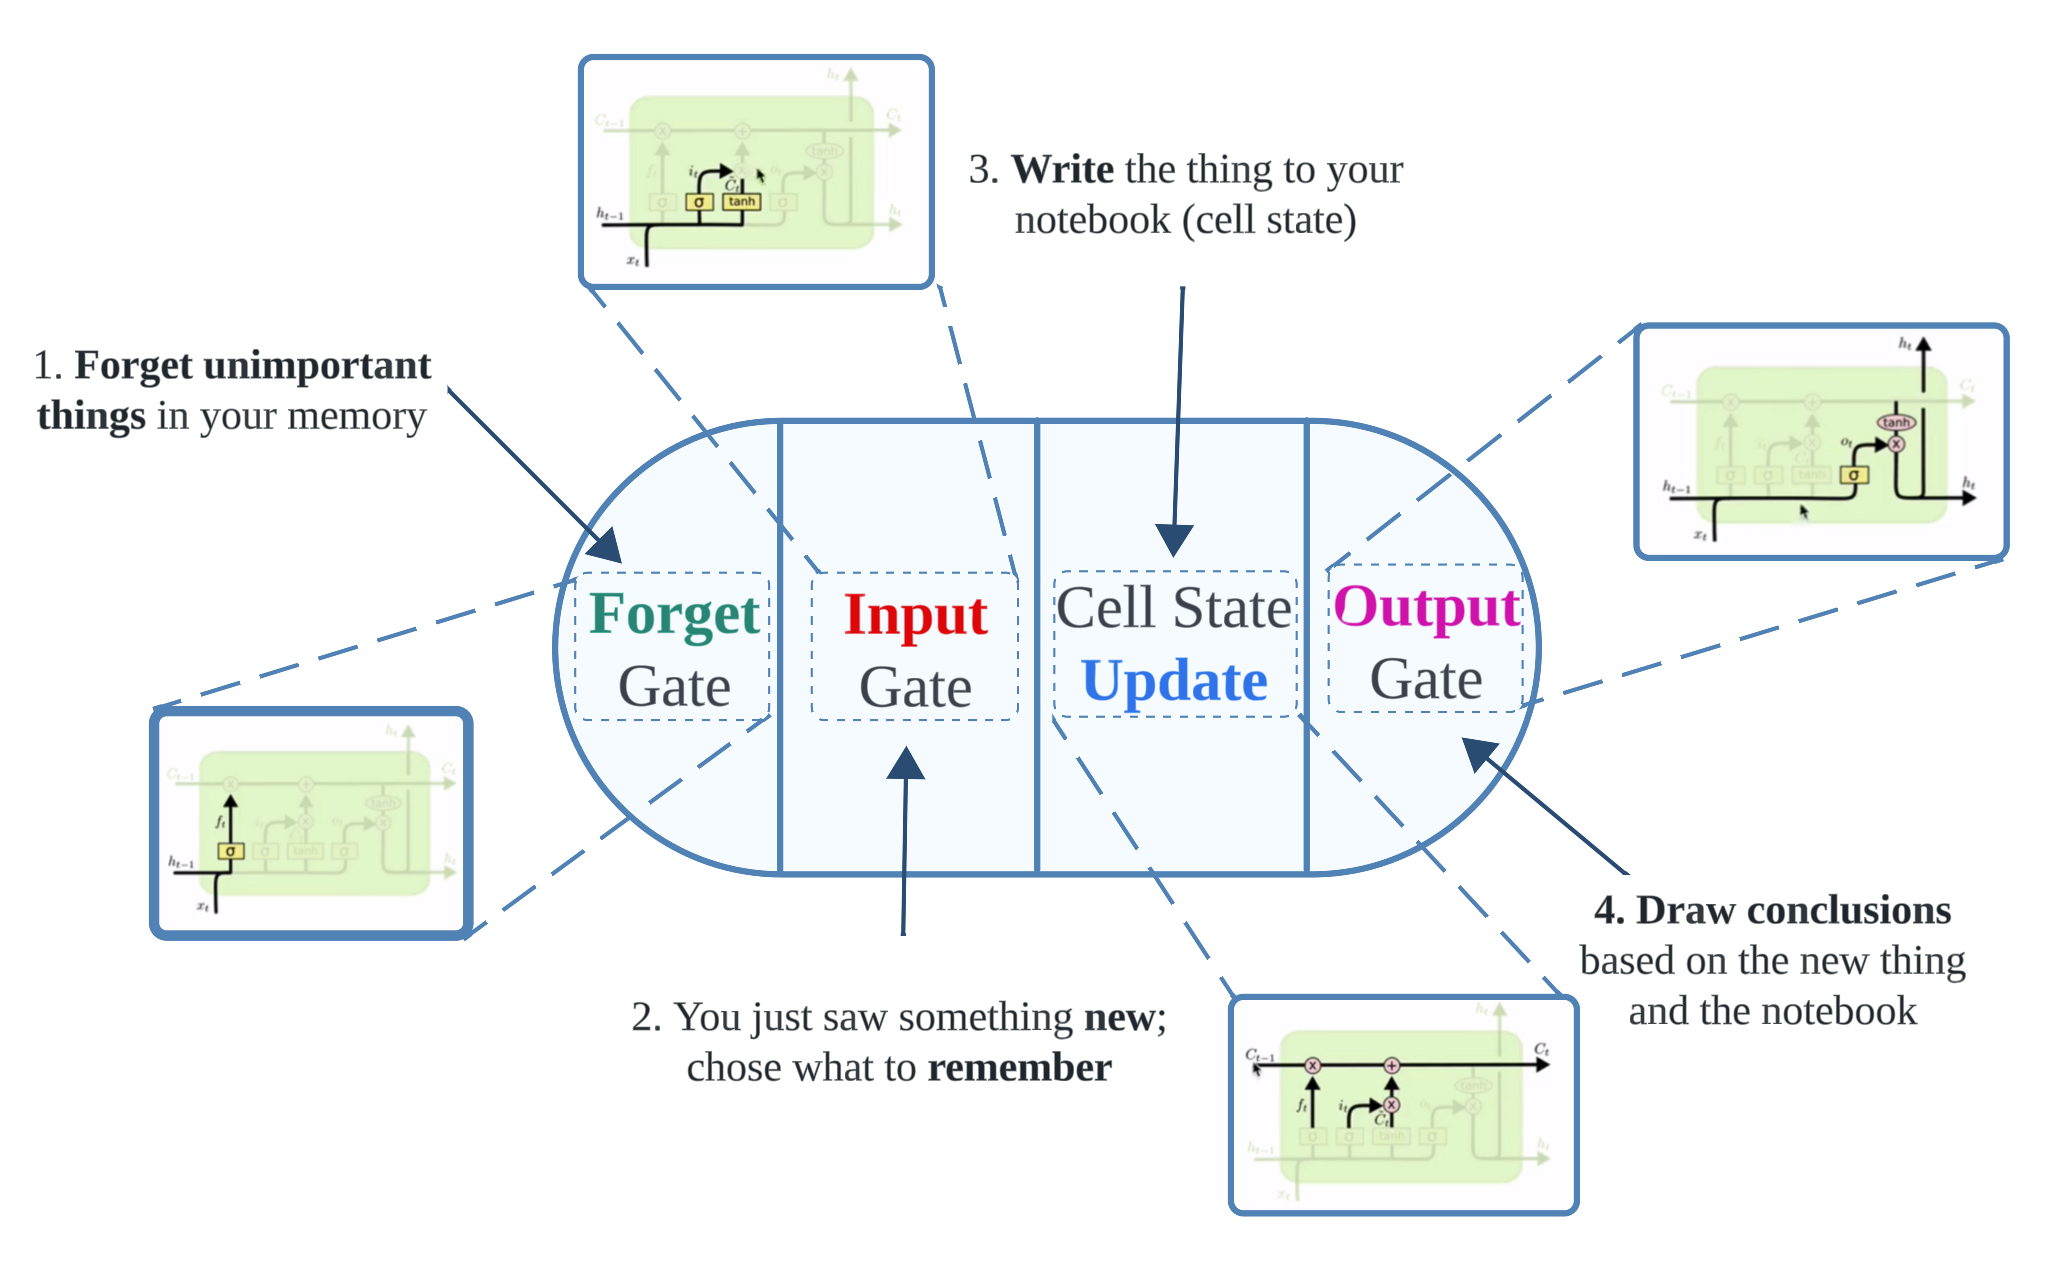
\includegraphics[width=.8\textwidth]{LSTM.png} %图片的名称或者路径之中有空格会出问题 
	\caption{Simplified Description of the Process within a LSTM cell \cite{12}} % 图片标题 
\end{figure}
\vspace{-0.2cm}

In our MoQ model, we succesfully integrated the 4S factors (Scoring, Service, Stamina, Slip) with the LSTM's structure. Each point in a match is represented as a multi-dimensional vector, where each dimension corresponds to one of the 4S factors. These vectors form a time series, serving as the input to the LSTM model:

\[ S = \{s^{(1)}, s^{(2)}, ..., s^{(n)}\} \]

where \( s^{(t)} = LSTM(x_1^{(t)}, x_2^{(t)}, ..., x_m^{(t)}) \) encapsulates the 4S factors at point \( t \), with \( x_1^{(t)}, x_2^{(t)}, ..., x_m^{(t)} \) representing the individual metrics within those factors, and \( LSTM \) symbolizing the LSTM's complex function that maps these inputs to an output. This complex function can be mathematically described as the following sequence $(2)$, with the \textbf{bold} symbols representing trainable parameters: 


\begin{enumerate}
	\centering
\item Forget Gate: \( f_t = \sigma(\mathbf{W_f} \cdot [h_{t-1}, x^{(t)}] + \mathbf{b_f}) \)
\item Input Gate: \( i_t = \sigma(\mathbf{W_i} \cdot [h_{t-1}, x^{(t)}] + \mathbf{b_i}) \)
\item Cell State Update: \( \tilde{C}_t = \tanh(W_C \cdot [h_{t-1}, x^{(t)}] + b_C) \)
\item Final Cell State: \( C_t = f_t \ast C_{t-1} + i_t \ast \tilde{C}_t \)
\item Output Gate: \( o_t = \sigma(\mathbf{W_o} \cdot [h_{t-1}, x^{(t)}] + \mathbf{b_o}) \)
\item Hidden State: \( h_t = o_t \ast \tanh(C_t) \)
\end{enumerate}
	
where \( \sigma \) denotes the sigmoid function (described at $(2)$), \( \ast \) represents element-wise multiplication, the square brackets in $[h_{t-1}, x^{(t)}]$ means concatenation (taking the two vectors and combining them into a single, longer vector), \( \mathbf{W} \) and \( \mathbf{b} \) are the weight and bias vectors used in each respective gate, \( h_{t-1} \) is the previous hidden state, \( x^{(t)} \) is the input vector at time \( t \), \( C_t \) is the current cell state, and the hyperbolic tangent function (\( \tanh \))  is given by:
\[ \tanh(x) = \frac{e^{x} - e^{-x}}{e^{x} + e^{-x}} \]

The LSTM structure above sets the foundation for our predictive momentum model. Now given a set a time-series 4S factors, we will attempt to train this model to meet the performance metric as described above.

\subsubsection{Model Training}
The training of the MoQ model requires structuring the data from the 30 matches (excluding the final match) into a format suitable for time-series analysis. First, each data point consists of the 4S factors for one player at a specific point in the match. The model used only the 4S factors of one of the players in the match, because we do not want the same performance metric to be repeatedly trained on different factors for different players. Then, each match is treated as a separate sequence for the LSTM to process. Within each match, the model iterates through the points (time steps) in sequential order, learning the patterns and dynamics of momentum as the match unfold. 

The training process adjusts the LSTM's parameters - the weights (\(\mathbf{W}\)) and biases (\(\mathbf{b}\)) of different gates, to minimize the distance between the model's predictions and the actual outcomes defined by our performance metric \( M^{(t)} \). This is accomplished through forward propagation of inputs (the 4S factors at a data point) through the model to generate momentum predictions, and then calculating the difference between these predictions and the actual momentum measured by the performance metric, and then backpropagating this error to adjust the model parameters. 

\paragraph{Forward Propagation}
After processing the input at $(1)$ to form a time-series, for each iteration, At the start of a match, the LSTM's hidden state \( h_0 \) and cell state \( C_0 \) are initialized to small random values. The model then processes the match point-by-point. For each point t, the 4S factors at that time step $s^{(t)}$ are fed into the LSTM as input. The LSTM updates its cell state based on this input and its previous states, producing an output that corresponds to the predicted momentum at that point, as described on $(3)$.

\paragraph{Back Propagation}
The model's predictions produced at the forward propagation phase are compared to the actual momentum metrics $M^{(t)}$ to calculate the loss, using a specific loss function. This loss is then backpropagated through the model to adjust the parameters, improving the model's predictions for the next iteration (point) within the match. We used the default optimizer and loss function of the TensorFlow framework. The detailed description for their implementation of LSTM can be found in \cite{13}.

So far we have thoroughly described the model structure and training process of MoQ. But is the model any good? Can it truly model the momentum? We will see them in the Experiment section below.




\section{Experiment}
In this section, we provide an validation of the MoQ model, testing its accuracy and provide a correlation analysis to show the model's capability to quantify momentum; moreover, we use the result of the model to predict flow of momentum, and see what can lead to the change on flow of play. 

\subsection{Model's Result on Quantifying Momentum}
The testing of MoQ involves predicting all 322 points (excluding the first 12 points) for the Wimbledon 2023 Men's Final, on Carlos Alcaraz (Player 1). We compared the LSTM's prediction results of momentum, to the actual performance metric that we designated. The result is illustrated in Figure .

\begin{figure}[htbp]  %h此处,t页顶,b页底,p独立一页,浮动体出现的位置
	\centering  %图表居中
	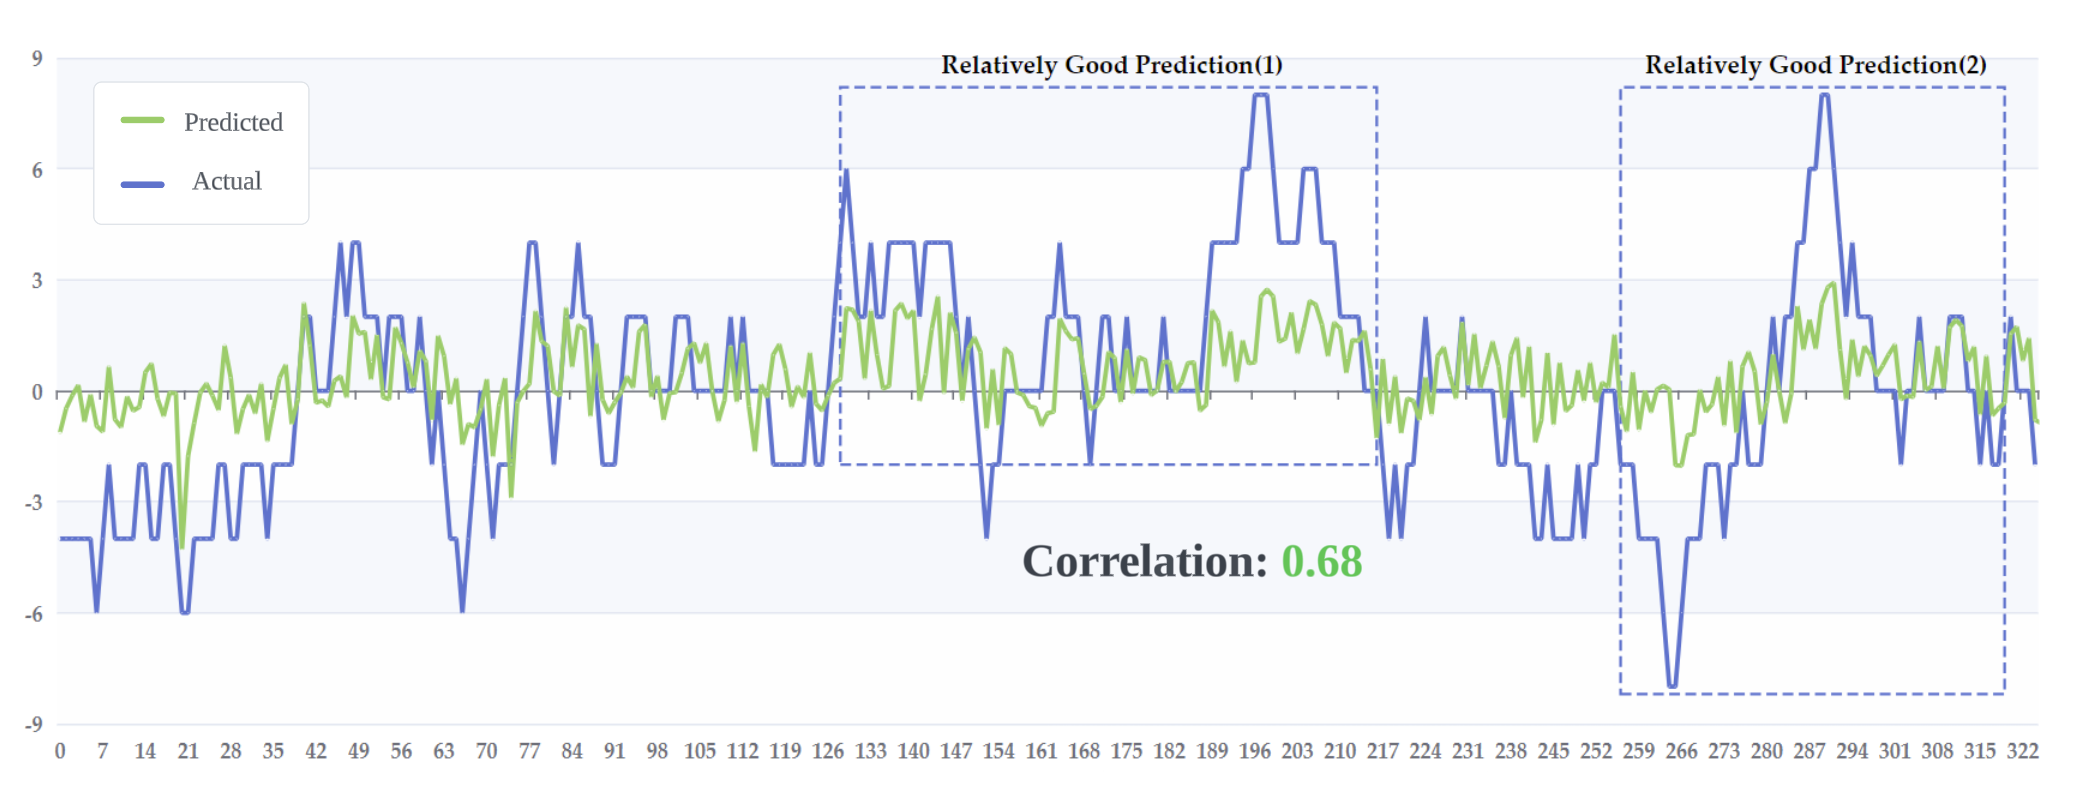
\includegraphics[width=\textwidth]{fluctuation.png} %图片的名称或者路径之中有空格会出问题 
	\caption{MoQ Prediction Result on the Final Match (excluding the first 12 points)} % 图片标题 
\end{figure}
\vspace{-0.2cm}

From the graph, we can judge that the model has a good predictive power on capturing when there's a significant shift of momentum, for example, the "Relatively Good Prediction" areas marked by the dashed lines. The model is mostly right in capturing the swings in momentum, although the momentum's volume between the prediction and actual is still large, as depicted in the figure. This could either due to the limitation of time-series analysis for being bad at predicting extreme values \cite{14}, or the unpredictability nature of momentum.

As mentioned in problem analysis, to measure whether this model is effective at predicting momentum, we have to conduct a correlation analysis between the performance metric and the predicted momentum value. The Pearson correlation coefficient, denoted as \( r \), providing a measure of the linear correlation between these two sets of data.

The Pearson correlation coefficient is defined as:

\[ r = \frac{\sum_{i=1}^{n} (s^{(t)} - \bar{s})(M^{(t)} - \bar{M})}{\sqrt{\sum_{i=1}^{n} (s^{(t)} - \bar{P})^2 \sum_{i=1}^{n} (M^{(t)} - \bar{M})^2}} \]
where \( s^{(t)} \) i is predicted momentum values at point \( t \), \( M^{(t)} \) represents the actual momentum metrics at point \( t \), \( \bar{s} \) and \( \bar{M} \) are the means of the predicted values and actual metrics, respectively, and \( n \) is the total number of points analyzed (322). After calculation, we found that the correlation between the performance metric and the result of the momentum model is exceptionally high: $\mathbf{0.68}$. This is out of our expectation because this means our model aligns well with the observable changes in the performance metric, meaning it has been successful at modeling momentum to some level, only using the limited data provided by the original problem! Most importantly, it indicates momentum can be a \textit{real thing} that affects the ebb and flow of the match!

\subsection{Are Shifts in Momentum Random?}
Now that we have a model that quantifies momentum, is there any indicator in the match that can predict a shift of momentum? To answer this this question, we have to first understand what is "a shift of momentum". Since our model is trained on using the average momentum of the 12 points after the predicting point, if at this point the value is significantly different than the last point's value, we can say that this point could potentially cause a shift of momentum and it will be reflected in the subsequent 12 points. Specifically, we can define a shift of momentum at point \( t \) if the absolute difference in the momentum values between point \( t \) and the previous point \( t-1 \) exceeds a certain threshold \( M_{\text{shift}} \). This can be expressed as:

\[ \Delta M^{(t)} = | M^{(t)} - M^{(t-1)} | > M_{\text{shift}} \]
where \( M^{(t)} \) is the calculated momentum value using MoQ at point \( t \), \( M^{(t-1)} \) is the momentum value at point \( t-1 \), \( M_{\text{shift}} \) is a predefined threshold that quantifies what constitutes a "significant" change in momentum. The choice of \( M_{\text{shift}} \) is important, which must be large enough to filter out minor fluctuations that are normal. Figure showed a distribution of $\Delta M$:

 \begin{figure}[htbp]  %h此处,t页顶,b页底,p独立一页,浮动体出现的位置
 	\centering  %图表居中
 	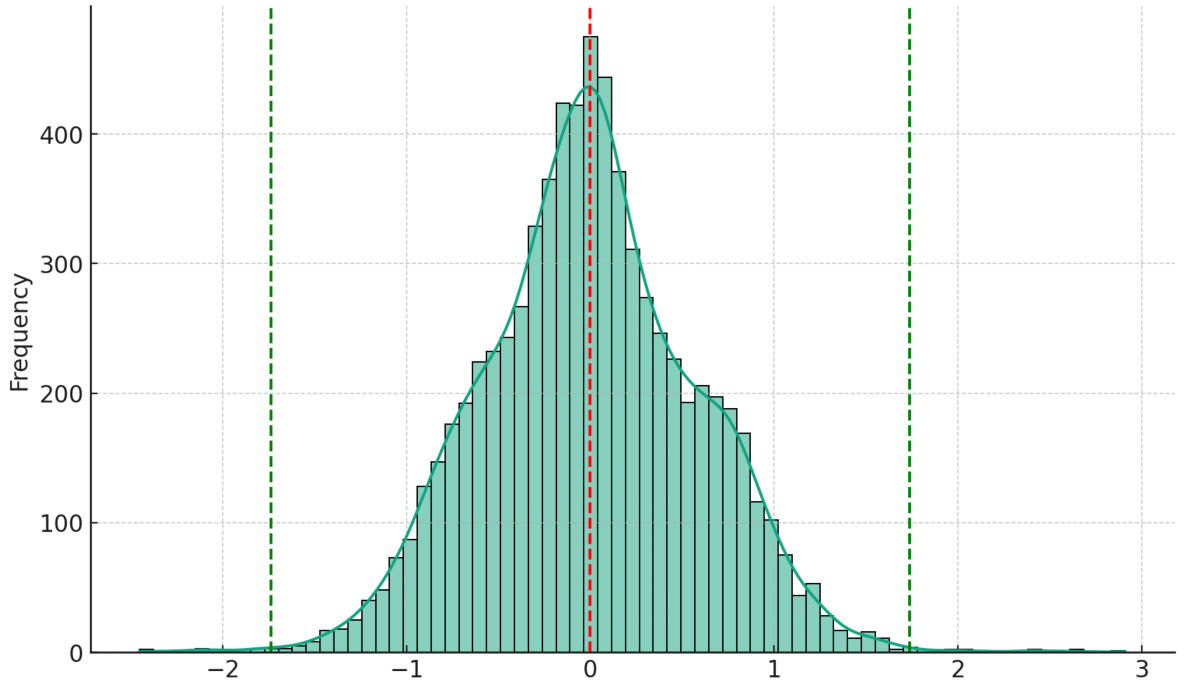
\includegraphics[width=0.6\textwidth]{range.png} %图片的名称或者路径之中有空格会出问题 
 	\caption{Distribution of value $\Delta M$} % 图片标题 
 \end{figure}
 \vspace{-0.2cm}
 
Initially it looked like a normal distribution, so we used a normal distribution test like Shapiro-Wilk's test (the detail of this testing can be found in \cite{15}). The calculation result, $\text{p-value} = 0.00031$, clearly rejected the null hypothesis of normality. With this result, we can already conclude that the shifts in momentum are not random. However, we still have to define the threshold $\Delta M$ to count for the data points that lead to a change in momentum. In statistics, the common way to set up such threshold is using the formula below:
\[ M_{\text{shift}} = k \times \sigma_{\Delta M} \]
where \( M_{\text{shift}} \) is the threshold for defining a significant shift in momentum, \( k \) is the multiplier that determines how stringent the threshold is, and \( \sigma_{\Delta M} \) is the standard deviation of the \( \Delta M \) values, representing the typical deviation from the average change in momentum. When assuming that distribution is normal, \( k = 2 \) is often selected to represent approximately the 95th percentile of a distribution. In our model where $\Delta M$ does not follow a normal distribution but resembles the shape, we can still use \( k = 2 \) to count the most significant shifts in momentum.

By applying this method to the whole dataset, we calculated $M_{\text{shift}} = 1.25698$, and accounted for a total of 694 points. This means when using our MoQ model to predict momentum, if the change of momentum $\Delta M^{(t)}$ at a timestep $t$ is larger than $1.25698$, a swing in the match might be happening.

Finally, using this 694 points, we try to filter the most important factors from the 4S factor that can cause a shift in momentum. This is done by using the correlation analysis, as defined in (), between the value of momentum change $\Delta M$ and the value of each of these factors in the 4S factors set. The result is described in the Figure .

We can interpret this result as the following: 
\begin{itemize}
	    \setlength{\parsep}{0ex} %段落间距
	\setlength{\topsep}{0ex} %列表到上下文的垂直距离
	\setlength{\itemsep}{0ex} %条目间距
	\item For the scoring factor, there is a strong positive correlation of 0.72, indicating the prediction results of our CourtSense model is moderately related to shifts in momentum. In other words, winning the current point is can be associated with a shift in momentum, but not every point winning leads to a momentum shift.
	\item The service factor has a moderate positive correlation of 0.49 with shifts in momentum. This suggests that factors related to service are moderately associated with momentum shifts. Specifically, aces having a correlation of 0.20 with momentum shifts, meaning scoring an ace has a little chance to cause a momentum shift.
	\item The stamina factor in total can have a good correlation with the shifts in momentum, but for individual factors, only the dist\_run (the total distance covered when playing that point) and rally count shows a weak negative correlation with the momentum shifts. This could be due to the fatigue during the match; hence we encourage the tennis coaches to focus on some amount of stamina training.
	\item The slip factor is pretty important in influencing the match's flow. We can see unforced errors have a moderate negative correlation of -0.42 with momentum shifts. Although not quite indicative of the player's performance, making unforced errors may be able to cause a psychological effect. Therefore, make sure to avoid unforced errors during the play of tennis.
\end{itemize}

Nonetheless, we cannot find a very important factor in the 4S factors correlations that has a high correlation with shifts in momentum. We believe this is due to the nature and complexity of momentum. Being able to find some moderate correlations, we believe, is good enough to provide insights to the help determine the changes in momentum.

\begin{figure}[htbp]  %h此处,t页顶,b页底,p独立一页,浮动体出现的位置
	\centering  %图表居中
	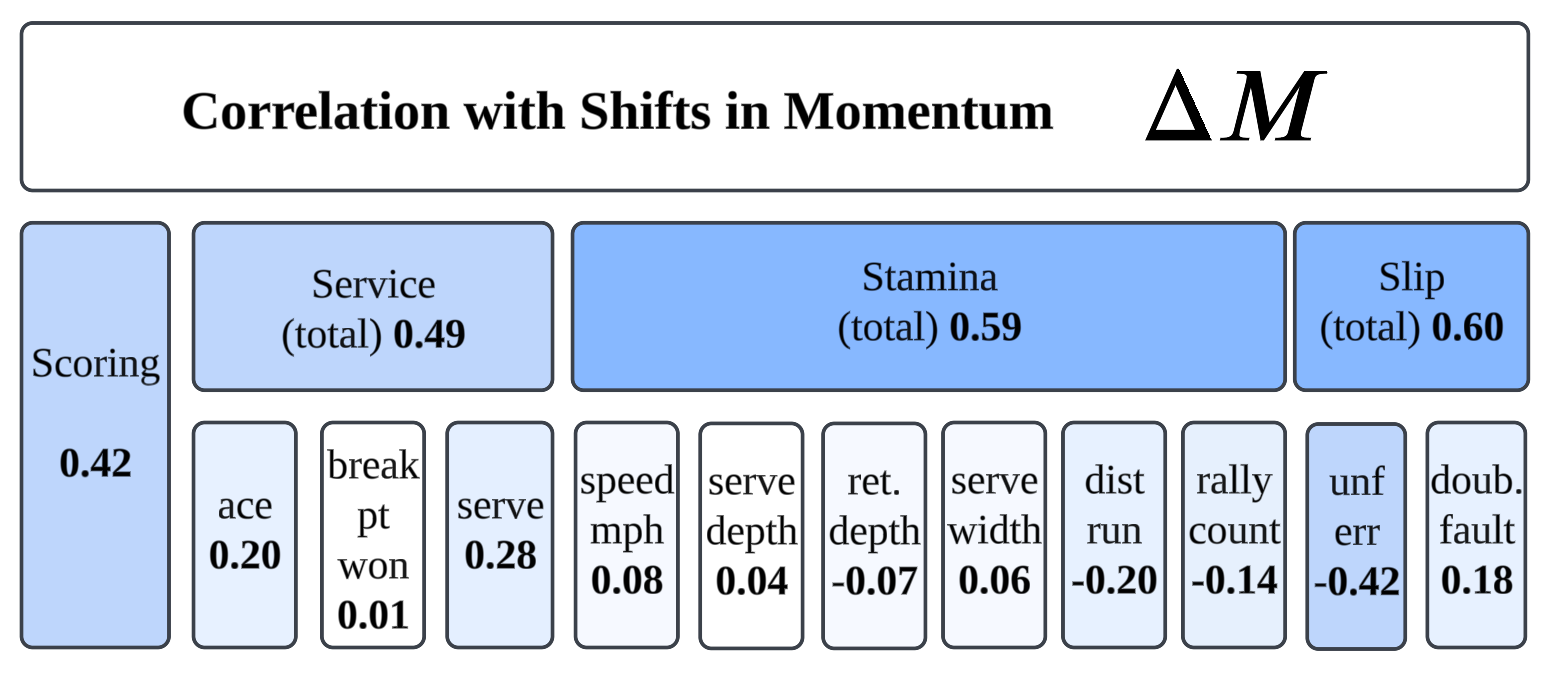
\includegraphics[width=0.85\textwidth]{correlation.png} %图片的名称或者路径之中有空格会出问题 
	\caption{Correlations between Change in Momentum with different 4S Factors. The total value is obtained by simple addition of the absolute values of individual factors in hope to capture the combined effect on momentum.} % 图片标题 
\end{figure}
\vspace{-0.2cm}

\subsection{On other matches: Generalizability Test}

Judging from the map of Victoria in Figure 4 (right), the eastern region is mainly forest, while the western region is almost no forest. Furthermore, to demonstrate better the situa-tion of wildfires, we plot over a heat map in Figure 4 (left).
Considering the heat map we made, it shows the number of wildfires in various states of Victoria from 2012 to 2021, the darker the color, the greater number of fires. Although fires have also occurred in the western region, the number of eastern regions is much higher than that in the western region. 

\begin{figure}[htbp]
    \centering    
    \subfigure[Data Screening(left)]{				% 图片1([]内为子图标题)						
    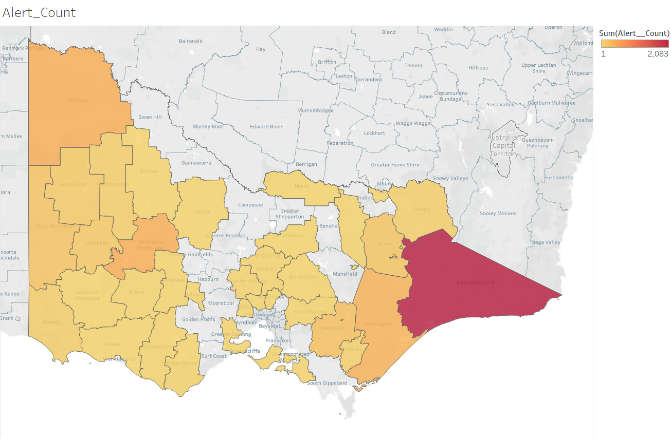
\includegraphics[width=0.45\textwidth]{Data_Screening(1).png}}			  % 子图1的图片宽度 不能空行
    \subfigure[Data Screening(right)]{				% 图片2
    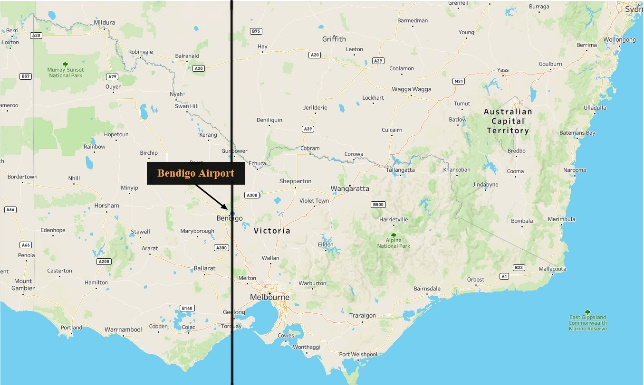
\includegraphics[width=0.45\textwidth]{Data_Screening(2).png}}
	\caption{Data Screening} % 图片标题 
\end{figure}

\begin{algorithm}
	\caption{BLAH BLAH BLAH}
	\begin{algorithmic}[1] % The [1] option enables line numbering
		\REQUIRE wordlist, gameround, v, r, f
		\ENSURE bestguess
		\STATE $pguesses \gets []$
		\STATE $freq \gets modfreq(wordlist)$
		\FOR{$i \gets 1$ \TO $length(wordlist)$}
		\STATE $w \gets weightings(wordlist[i], freq, v, r, f)$
		\STATE $pguesses.append([w, wordlist[i]])$
		\ENDFOR
		\STATE $pguesses.sort(reverse = True)$
		\RETURN $pguesses[0][1]$
	\end{algorithmic}
\end{algorithm}


\begin{table}[htbp]
	\begin{center}
		\caption{Data and Database Websites}
		\resizebox{\textwidth}{!}
		{\begin{tabular}{c c}
				\toprule[2pt]
				\multicolumn{1}{m{5cm}}{\centering \textbf{Database Names}}
				&\multicolumn{1}{m{10cm}}{\centering \textbf{Database Websites} }\\ %m后面是列宽
				\midrule
				Fire Alerts& https://www.globalforestwatch.org/map/ \\
				Altitude & https://search.earthdata.nasa.gov/search \\
				Latitude and Longitude & https://www.kaggle.com/carlosparadis/\\ 
				Google Scholar & https://scholar.google.com/ \\
				Maps& \copyright{} 2021 Mapbox \copyright{} OpenStreetMap\\
				\bottomrule[2pt]
		\end{tabular}}
	\end{center}
\end{table}



% F: References & Appendix

\clearpage   
\begin{thebibliography}{99}
	\bibitem{-1} \href{https://www.sportsperformancebulletin.com/psychology/psychological-aides/the-role-of-momentum-in-sports-performance}{Andrew Hamilton, Psychological Aides Sector, Sports Performance Bulletin. The Role of Momentum in Sports Performance.}
    \bibitem{1} \href{https://www.skysports.com/tennis/news/32498/12920986/wimbledon-carlos-alcaraz-dismantles-daniil-medvedev-to-set-up-final-against-novak-djokovic}{Skysports | Wimbledon: Carlos Alcaraz dismantles Daniil Medvedev to set up final against Novak Djokovic.}
	\bibitem{2} \href{https://medium.com/swlh/cde03d99f410}{Medium | Predicting ATP Tennis Match Outcomes Using Serving Statistics.}
	\bibitem{3} \href{https://www.princeton.edu/~dixitak/home/Tennis.pdf}{Avinash Dixit, Susan Skeath. The Most Important Situations in Tennis – and in R\&D Competition.}
	\bibitem{4} \href{https://www.cis.upenn.edu/~bhusnur4/cit592\_fall2013/NeKe2005.pdf}{Pual K. Newton, Joseph B. Keller. Probability of Winning at Tennis I. Theory and Data.}
	\bibitem{5} \href{https://papers.tinbergen.nl/02119.pdf}{JS Cramer, University of Amsterdam, 2022. The Origins of Logistic Regression. }
	\bibitem{6} \href{https://www.analyticsvidhya.com/blog/2021/07/metrics-to-evaluate-your-classification-model-to-take-the-right-decisions/}{Analytics Vidhya | Metrics to Evaluate your Classification Model.}
	\bibitem{7} \href{https://www.youtube.com/watch?v=5uFAkizQNJI}{A FINAL FOR THE AGES | Carlos Alcaraz vs Novak Djokovic Full Match | Wimbledon 2023}
	\bibitem{8} \href{https://www.researchgate.net/publication/318275570_Momentum_in_tennis_Controlling_the_match}{Helmut Dietl, Cornel Nesseler, University of Zurich, 2017. Momentum in tennis: Controlling the match}
	\bibitem{9} \href{https://www.tandfonline.com/doi/full/10.1080/02701367.2019.1666203}{Min Kyu Sim, Dong Gu Choi, Pohang University of Science and Technology, 2019. The Winning Probability of a Game and the Importance of Points in Tennis Matches}
	\bibitem{10} \href{https://arxiv.org/pdf/1701.01887.pdf}{John Gamboa, University of Kaiserslautern, 2017. Deep Learning for Time-Series Analysis. arXiv:1701.01887v1}
	\bibitem{11} \href{https://ieeexplore.ieee.org/document/9420543}{Reza Ghanbari, Keivan Borna, IEEE, 2021. Multivariate Time-Series Prediction Using LSTM Neural Networks.}
	\bibitem{12} \href{https://www.analyticsvidhya.com/blog/2021/03/introduction-to-long-short-term-memory-lstm/}{Analytics Vidhya | Shipra Saxena, What is LSTM? Introduction to Long Short-Term Memory}
	\bibitem{13} \href{https://github.com/keras-team/keras/blob/v2.15.0/keras/layers/rnn/lstm.py#L382-L891}{Github | keras/keras/layers/rnn/lstm.py at v2.15.0 · keras-team/keras}
	\bibitem{14} \href{https://arxiv.org/pdf/2012.10763.pdf}{Han Lin Shang, Macquarie University; Ruofan Xu, Monash University, 2020. Functional time series forecasting of extreme values. arXiv:2012.10763v1}
	\bibitem{15} \href{https://en.wikipedia.org/wiki/Shapiro%E2%80%93Wilk_test}{Wikipedia | Shapiro–Wilk test}

\end{thebibliography}

% Letter Page

\clearpage
\pagestyle{fancy}
\fancyhead{} % Clear all header fields
\begin{letter}{Letter to Central Intelligence Agency}
	\textbf{}\\
	\textbf{To:} Recipient Name \\
	\textbf{From:} Your Name \\
	\textbf{Subject:} The Subject of Your Letter \\
	\textbf{Date:} \today \\
	\textbf{}
	\begin{multicols}{2}
	We want to develop and summarize a model to classify solution words by difficulty.We constructed an AI
	simulating human thinking to solve problems based
	on iterative optimization parameter finding strategy.
	It could solve wordle about 3 times on average. We
	trained 450 such AI and took the average number of
	solving problems as the evaluation standard of difficulty. After that, we used k-means clustering algorithm
	to successfully classify normal problems and difficult
	problems, and found that normal problems generally
	have the characteristics of high word frequency, small
	number of non-repeating letters and so on.We also used
	correlation analysis to assess the relationship between
	the ai difficulty prediction and the average number
	of problems solved by humans, which showed a significant correlation. This verifies the accuracy of our
	model.
	Finally, we visualized the data and found an interesting conclusion: although daily reported results decreased, the proportion of difficult patterns increased.
	We attribute this to the presence of strong old players
	and a reluctance to post simple reports.We also found
	that the number of non-repeating letters also affected
	the percentage of hard mode.
	That’s all from our data analysis. I hope it’s helpful
	to your game. Thanks for watching.
	\end{multicols}
	
\end{letter}



% AI Report Page

\newcounter{savedpage}
\setcounter{savedpage}{\value{page}}

\includepdf[pages=-]{AIreport.pdf} 
\setcounter{page}{\value{savedpage}}

\end{document}  % 结束